% !TEX encoding = UTF-8
% !TEX TS-program = pdflatex
% !TEX root = ../Relazione.tex
% !TEX spellcheck = it-IT
\clearpage
\section{Teoria delle reti}
\label{sec:teoria}
Le reti sono insiemi di oggetti per i quali è possibile una connessione. Gli ultimi 60 anni hanno visto un crescente interesse per esse, perché con le reti è possibile descrivere sistemi dei più disparati tipi nei campi più vari, dalla biologia all'economia, passando per reti elettriche, informatiche, ecosistemi,  e altro ancora. Ancora più importante, negli ultimi vent'anni è stato scoperto che una classe di reti ha proprietà del tutto comuni nonostante l'intrinseca diversità tra sistemi; la modellizzazione di queste reti, come crescita con caratteristiche preferenziali, è dovuta a \textcite{Barbalbert1999}, e vengono dette scale-free.

Per maggior semplicità, nell'esposizione del lavoro svolto verrà sempre assunto che le reti siano dirette e non pesate.

\subsection{Proprietà e grandezze caratteristiche}
Dal punto di vista matematico una rete è rappresentata da un grafo. Gli oggetti costitutivi di un grafo sono i \textbf{nodi}, i quali vengono collegati opportunamente tra loro con dei \textbf{link} secondo dei criteri che dipendono dal modello (nella costruzione di un grafo teorico) o dalla natura del sistema (per le reti reali). Il numero di nodi della rete, o di una sua parte, è ovviamente la grandezza fondamentale per definirne le dimensioni; il numero e la distribuzione dei link ne descrivono la connettività.

Prima di procedere alla descrizione dei modelli di rete sopracitati, è utile elencare un glossario di caratteristiche delle reti, spesso determinanti per distinguere un grafo scale-free dagli altri nello studio delle reti reali.

\begin{description}
	\item[Grado] Il grado di un nodo è il numero di altri nodi a cui è connesso. La connettività di una rete è ben rappresentata dalla \textbf{distribuzione del grado}, la cui forma funzionale $P(k)$ la cui forma funzionale è il primo criterio per discriminare una rete scale-free. 
	
	\item[Distanze] alla base di ogni topologia c'è il concetto di distanza. La distanza tra due nodi di un grafo è definita come il numero di link che li separa nel più piccolo cammino possibile lungo la rete. Altre quantità topologiche importanti sono:
	\begin{itemize}
		\item l'\textbf{eccentricità di un nodo}, è la massima delle distanze tra un nodo scelto e tutti gli altri nodi della rete;
		\item il \textbf{diametro} è la massima eccentricità tra quelle di tutti i nodi del grafo; detto in termini più generali, il diametro è il minor cammino più grande tra tutte le possibili coppie di nodi della rete;
		\item \textbf{average path length}, cio\`e la distanza media tra tutte le possibili coppie di nodi della rete.
	\end{itemize} 
%TODO (correlazione con diametro?)-->
	
	\item[Custering] Per misurare quanto i nodi di un grafo tendono a creare dei clusters, viene definito il coefficiente di clustering $C_i$. Dal punto di vista di un vertice $i$ di grado $k_i$, quindi, considerando i nodi a esso collegato, $C_i$ è definito come il rapporto
	\[C_i = \frac{2E_i}{k_i(k_i-1)},\]
	dove $E_i$ è il numero di link tra i $k_i$ primi vicini del vertice e $k_i(k_i-1)/2$ il numero di link possibili tra essi: cioè il numero di collegamenti necessari perché $i$ con i suoi vicini sia una porzione di grafo \emph{completa}, detta anche \emph{clique}.  
	La media su tutti i nodi dei rispettivi $C_i$ dà un'indicazione su quanto la rete sia complessivamente clusterizzata e quindi può essere preso come coefficiente di clustering globale $C$ della rete. Una definizione più recente di $C$, equivalente alla precedente, lo pone uguale al rapporto tra il numero di triplette di nodi completamente collegate $N_\triangle$ e il numero di triplette che vede i tre nodi collegati da almeno due link $N_\wedge$. In entrambi i casi, più $C$ è vicino a $1$, più si ha clusterizzazione.
	
	Il coefficiente di clustering svolge un ruolo importante nel distinguere una rete completamente random da una che presenta caratteristiche di \emph{small-world}: infatti un rete con piccolo diametro tende a avere un $\langle C\rangle$ maggiore di una simile rete puramente casuale costruita con lo stesso numero di nodi e con il medesimo cammino più corto medio. Questo comportamento è stato notato in molte reti reali \parencite{Watts1998}.
	\item[Centralit\`a] Esistono vari modi per definire quando un nodo è centrale rispetto ad altri. Il primo è più immediato è il suo grado. Altri due tra i più importanti sono la \textbf{betweenness} e il \textbf{page-rank}. Preso un nodo $i$, il primo è definito come il numero di cammini più corti che è possibile tracciare tra due qualsiasi nodi della rete, purché passino per $i$; il secondo dà una maggior centralità a $i$ maggiore è il numero di link \emph{diretti} verso di esso, tenendo conto anche del rank dei nodi che si collegano a esso. 
	
	In reti dirette, benché non siano \emph{matematicamente} uguali, betweenness e page-rank sono statisticamente molto correlati al grado, pertanto non verranno analizzati. 
% 	TODO (fare grafico correlazione grado-betweenness-pagerank)
\end{description}

\subsection{Costruzione della rete e matrice di adiacenza}
Prese le antenne nell'area selezionata come i nodi della rete, è necessario definire un criterio per stabilire un link. Nell'ottica di una ipotetica mesh network, la scelta è stata di considerare collegate due antenne se non hanno zone d'ombra del segnale nello spazio tra di esse, in modo che qualsiasi utente al suo interno possa comunicare con altri utenti (si suppone quindi un diverso metodo di comunicazione tra antenne, come cavo, altri canali Wi-fi). Trascurando dislivelli del terreno e edifici, è stato supposto che la porzione di spazio coperta da un'antenna sia un cilindro del raggio fornito dai dati. Il criterio scelto è stato quindi che la distanza $\delta_{ij}$ tra due antenne fosse minore dei loro raggi in modo tale che essi si sovrappongano per il $20\%$: $\delta_{ij} < 0.8(r_i+r_j)$.

Stabilito il criterio, bisogna costruire la rete, popolando la matrice di adiacenza dei nodi. Dato che il criterio di linking richiede la conoscenza della distanza tra due antenne, è stato necessario calcolare le distanze tra ogni coppia di nodi. I dati in nostro possesso forniscono le coordinate geografiche, che sono delle coordinate sferiche, e quindi ci si è posti il problema di come calcolare le distanze. Inizialmente la scelta è caduta su una funzione della libreria geopy, la quale permette di calcoalare la distanza geodesica con il metodo great-circle e con la formula vincenty. La prima è più veloce e usa un modello sferico di Terra, la seconda richiede più calcoli perché usa un accurato modello ellissoidale (impiega circa il doppio del tempo del metodo great-circle). Purtroppo, tuttavia, i tempi di calcolo richiesti da queste funzioni sono piuttosto alti in prospettiva di calcolare una matrice di $7000^2$ elementi. 

Per risparmiare tempo, dato che la rete definita non è diretta, per prima cosa è stata modificata la funzione di calcolo della matrice di adiacenza in modo che calcolasse soltanto la metà superiore. Successivamente si poteva tentare di diagonalizzare a blocchi la matrice, cosa purtroppo impossibile poiché dai dati risulta che un certo numero di antenne hanno raggi d'azione nell'ordine dei 10-20 km, ricoprendo quindi tutta l'area di Roma selezionata. L'unica via praticabile per far calare drasticamente il tempo necessario per calcolare tutte le matrici necessarie per l'analisi è stata quindi convertire le coordinate geografiche in cartesiane e usare la distanza euclidea. In questo modo si è ottenuto un guadagno di velocità di un fattore 10. Calcolate le matrici definitive per la rete complessiva e per quelle delle singole compagnie, sono state salvate su file in modo da non doverle più ricalcolare.


\subsection{Distribuzione del grado}
I vettore di gradi per ogni nodo del grafo si ottiene con il metodo \lstinline{.degree()} della classe Graph di networkx. Abbiamo dunque fatto un istogramma congiunto di tutti i provider e della rete totale con un canale per ogni possibile numero naturare, ma in scala log-log risultava illegibile. Per ridurre un poco il rumore sulle code la canalizzazione è stata ridutta di 8 volte rispetto alle unità naturali. Data la poca estensione delle curve ed il fatto che molte non arrivavano fino ad 1, si è scelto di evitare il log-binning in base 2, in quanto in questo caso troppo grossolano e non in grado di conservare tutta l'informazione sulle code della distribuzione.

\begin{figure}[b!]
	\centering
	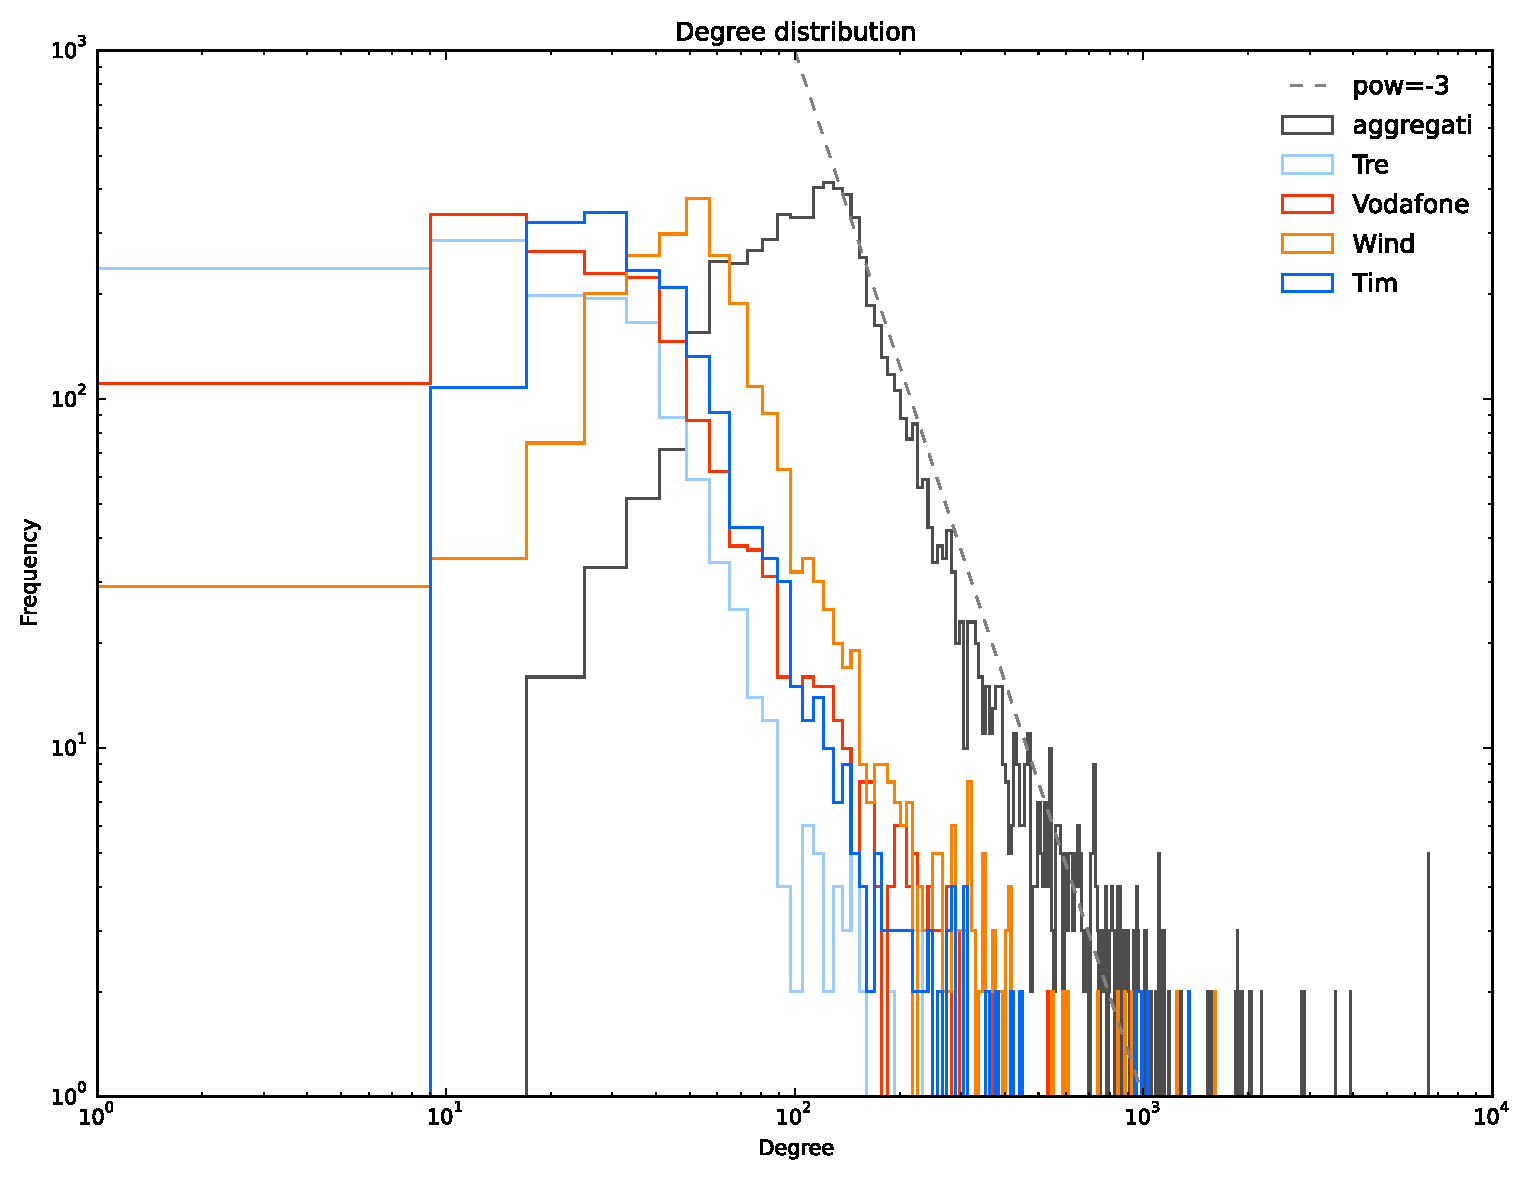
\includegraphics[width=0.8\textwidth]{./Immagini/Dati/degreeDistribution}
	\caption{Distribuzione dei gradi per le 5 reti analizzate}
	\label{fig:gradi}
\end{figure}

Come si può vedere nella figura \ref{fig:gradi}, soprattutto per la rete complessiva l'andamento è circa power law dal massimo in poi. L'esponente è in valore assoluto di poco superiore a 3 nella prima parte e di poco inferiore a 3 nell'ultima parte della coda, estesa per circa mezza decade.

In figura \ref{fig:kfreqrank} viene anche riportato l'andamento del frequency-rank (in forma di scatterplot per migliorarne la legibilità). La differenza nei valori sulle y rispetto all'istogramma precedente è dovuta al fatto che grazie all'ottima visibilità qui è stato possibile riprendere la canalizzazione sui numeri naturali, non aggregata.

\begin{figure}[t]
	\centering
	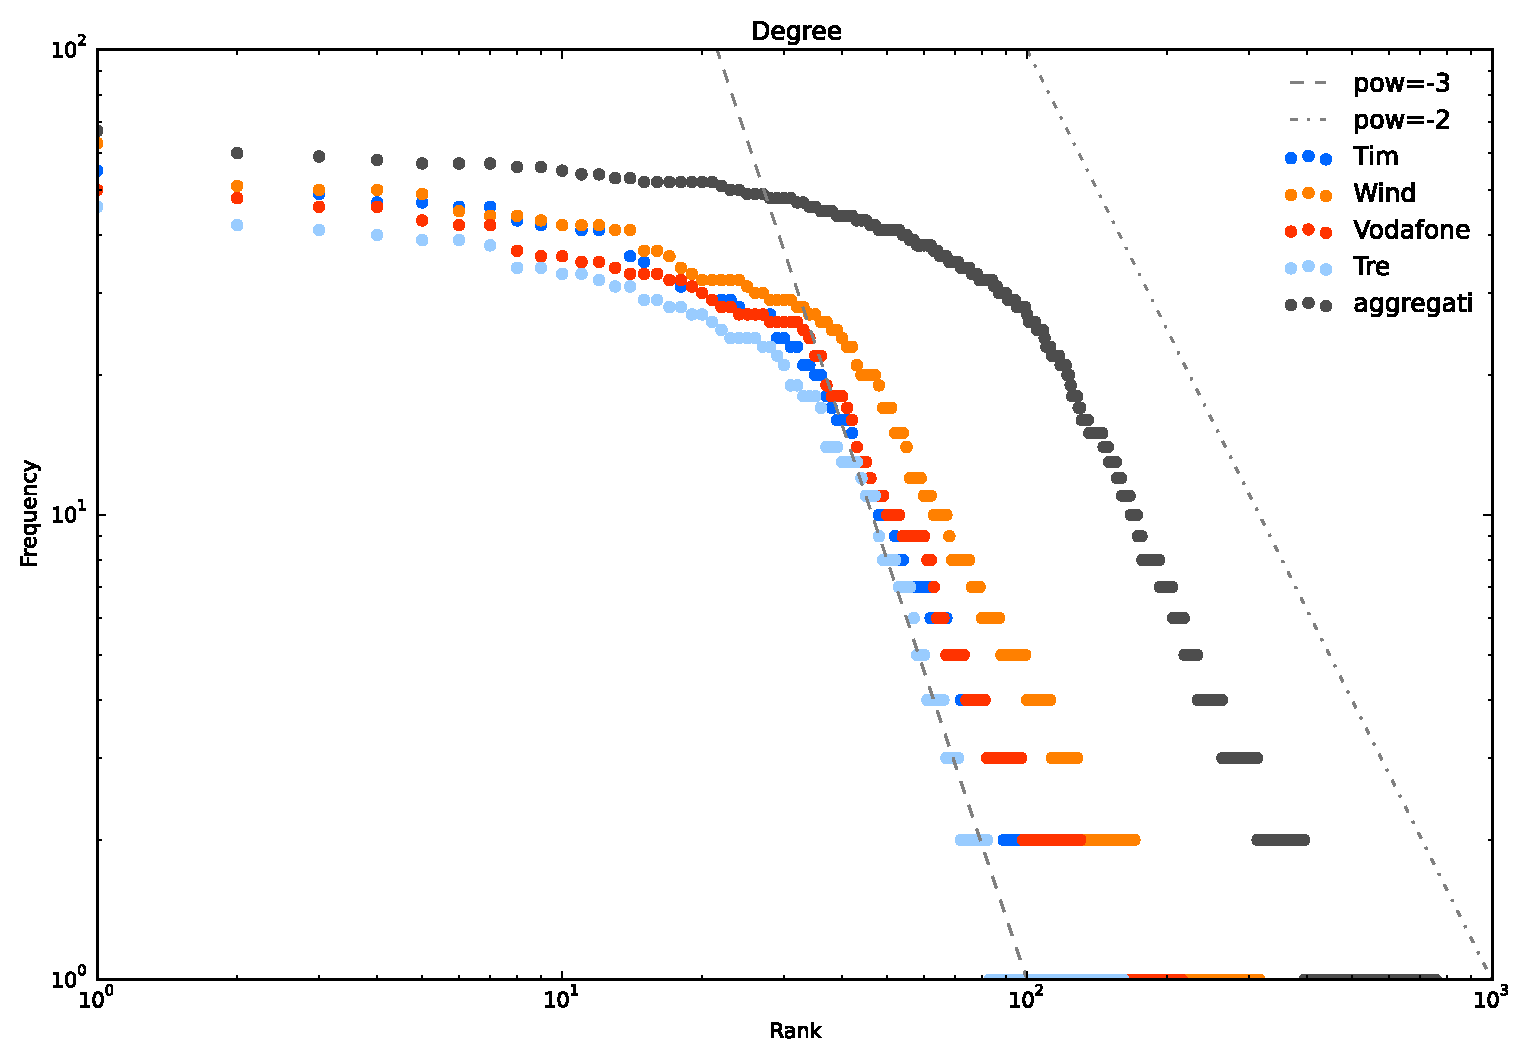
\includegraphics[width=0.8\textwidth]{./Immagini/Dati/kfreqrank}
	\caption{Frequency rank dei gradi per le 5 reti analizzate}
	\label{fig:kfreqrank}
\end{figure}

\subsection{Modelli di rete}
Costruite le reti e individuate le distribuzioni del grado che le caratterizzano, è utile avere alcuni importanti modelli di rete come paragone.

Lo studio delle reti random nasce dagli ungheresi \textcite{Erdos1959}, i quali per primi modellizzarono la definizione di una rete usando criteri probabilistici. Nel corso dei 40 anni successivi è stato osservato che molte reti reali, a dispetto delle dimensioni, avessero un diametro molto piccolo, portando alla definizione del concetto di \emph{small-worlds} e al modello di \textcite{Watts1998}.

In entrambi i casi si parte da una configurazione iniziale di nodi per poi randomizzare i link tra essi. Per questo motivo la distribuzione del grado segue una Poissoniana, con una coda destra caratteristica di forma esponenziale; con un numero sufficiente di nodi e link, la distribuzione del grado si approssima a una gaussiana con un grado medio ben definito.

\subsubsection{Random network}
Il modello di Erdős e Rényi parte da un certo numero $N$ di nodi e $n$ di link. Se poniamo che i nodi siano distinguibili, possono esistere $\binom{n}{N(N-1)/2}$ 
%TODO DA CONTROLLARE NUM CONF POSS, DISTINGUIBILITÀ-->
configurazioni equiprobabili tra le quali può esserne presa una in maniera random. Una maniera più articolata per definire una rete random è il criterio binomiale: partire da un set di $N$ nodi e dare a ogni possibile coppia un link con una certa probabilità  $p$. 
% TODO VALUTARE SE TENERE SOLO QUESTA DEFINIZIONE-->
Il punto più importante di un approccio probabilistico alle reti è lo studio di proprietà dei grafi: ponendo $N \rightarrow \infty$, se la probabilità che una certa proprietà si verifichi tende a 1, si osserva che per reti limitate quella proprietà si verifica con probabilità significativa anche con pochi nodi. Ciò si verifica per molte proprietà, e questo fatto permette di poter trattare le reti per categorie secondo le loro proprietà peculiari.

Nel caso di un grafo di Erdős e Renyi queste sono:

\begin{itemize}
	\item la distribuzione del grado ha una forma di distribuzione binomiale, la quale tende a una poissoniana per $p$ piccole, e a una gaussiana per $\langle k \rangle$ grandi. Questo implica che la topologia della rete è abbastanza omogenea, con molti nodi che hanno approssimativamente lo stesso grado;
	
	\item con $N$ grande, il diametro tende a essere piccolo, come l'average path length. Con $p$ non troppo piccolo il numero di nodi che abbiano una certa distanza una lunghezza $l$ si può approssimare a $\langle k\rangle^l$; uguagliandolo a $N$ deriva che diametro e average path length scalano con buona approssimazione con il logaritmo di N, secondo la relazione
	\begin{equation}
	\label{eq:lunghezze}
	l \sim \frac{ln(N)}{ln(\langle k \rangle)}. 	 
	\end{equation}
	Molte reti reali presentano simili caratteristiche nei gradi di separazione, che hanno portato alla definizione del termine "small world" per esse;
	
	\item il clustering di una rete ramdom tende a essere molto basso. Infatti, preso un nodo e i suoi primi vicini, la probabilità una coppia di essi sia connessa è $p$. Pertanto su tutto il grafo, il coefficiente di clustering medio è proprio $p$, il quale di solito è abbastanza minore di 1 (con $p = 0.1$ un grafo random diventa già molto connesso, per esempio con $10^4$ nodi avrebbe $\langle k\rangle = 10^3$). Questo fatto, al contrario del diametro, si pone in contrasto con le reti reali, le quali hanno quasi sempre un $\langle C \rangle$ sensibilmente più alto.
\end{itemize}

% \begin{wrapfloat}{figure}{I}{0pt}
% 	\centering
% 	\includegraphics[width=0.48\textwidth]{./Immagini/figureSpettro/fluoFe2}
% 	\caption[Emissione X del ferro]{Particolare dello spettro acquisito che mostra il fit con doppia gaussiana del picco studiato, ipoteticamente X del Fe.}
% 	\label{fig:fluoXFe}
% \end{wrapfloat}

\subsubsection{Small World}
Come abbiamo visto il modello di Erdős e Renyi descrive bene il piccolo diametro delle reti reali, ma non il loro elevato grado di clusterizzazione. Inoltre il coefficiente di clustering di esse è simile per reti con numero di nodi molto diverso. Notando per primi ciò, Watts e Strogatz hanno formulato un modello che meglio si adattasse alle caratteristiche reali delle reti. 

Il fatto che il coefficiente di clustering non dipende dal numero di nodi è caratteristico dei reticoli, pertanto il punto di partenza del modello di Watts e Strogatz è un reticolo con condizioni al contorno cicliche, i cui $N$ nodi sono collegati ai primi $n$ vicini. Se poniamo, per esempio, $n = 2$, si configura così un anello come in Figura \ref{fig:ring}.
\clearpage
\begin{figure}[t]
	\centering
	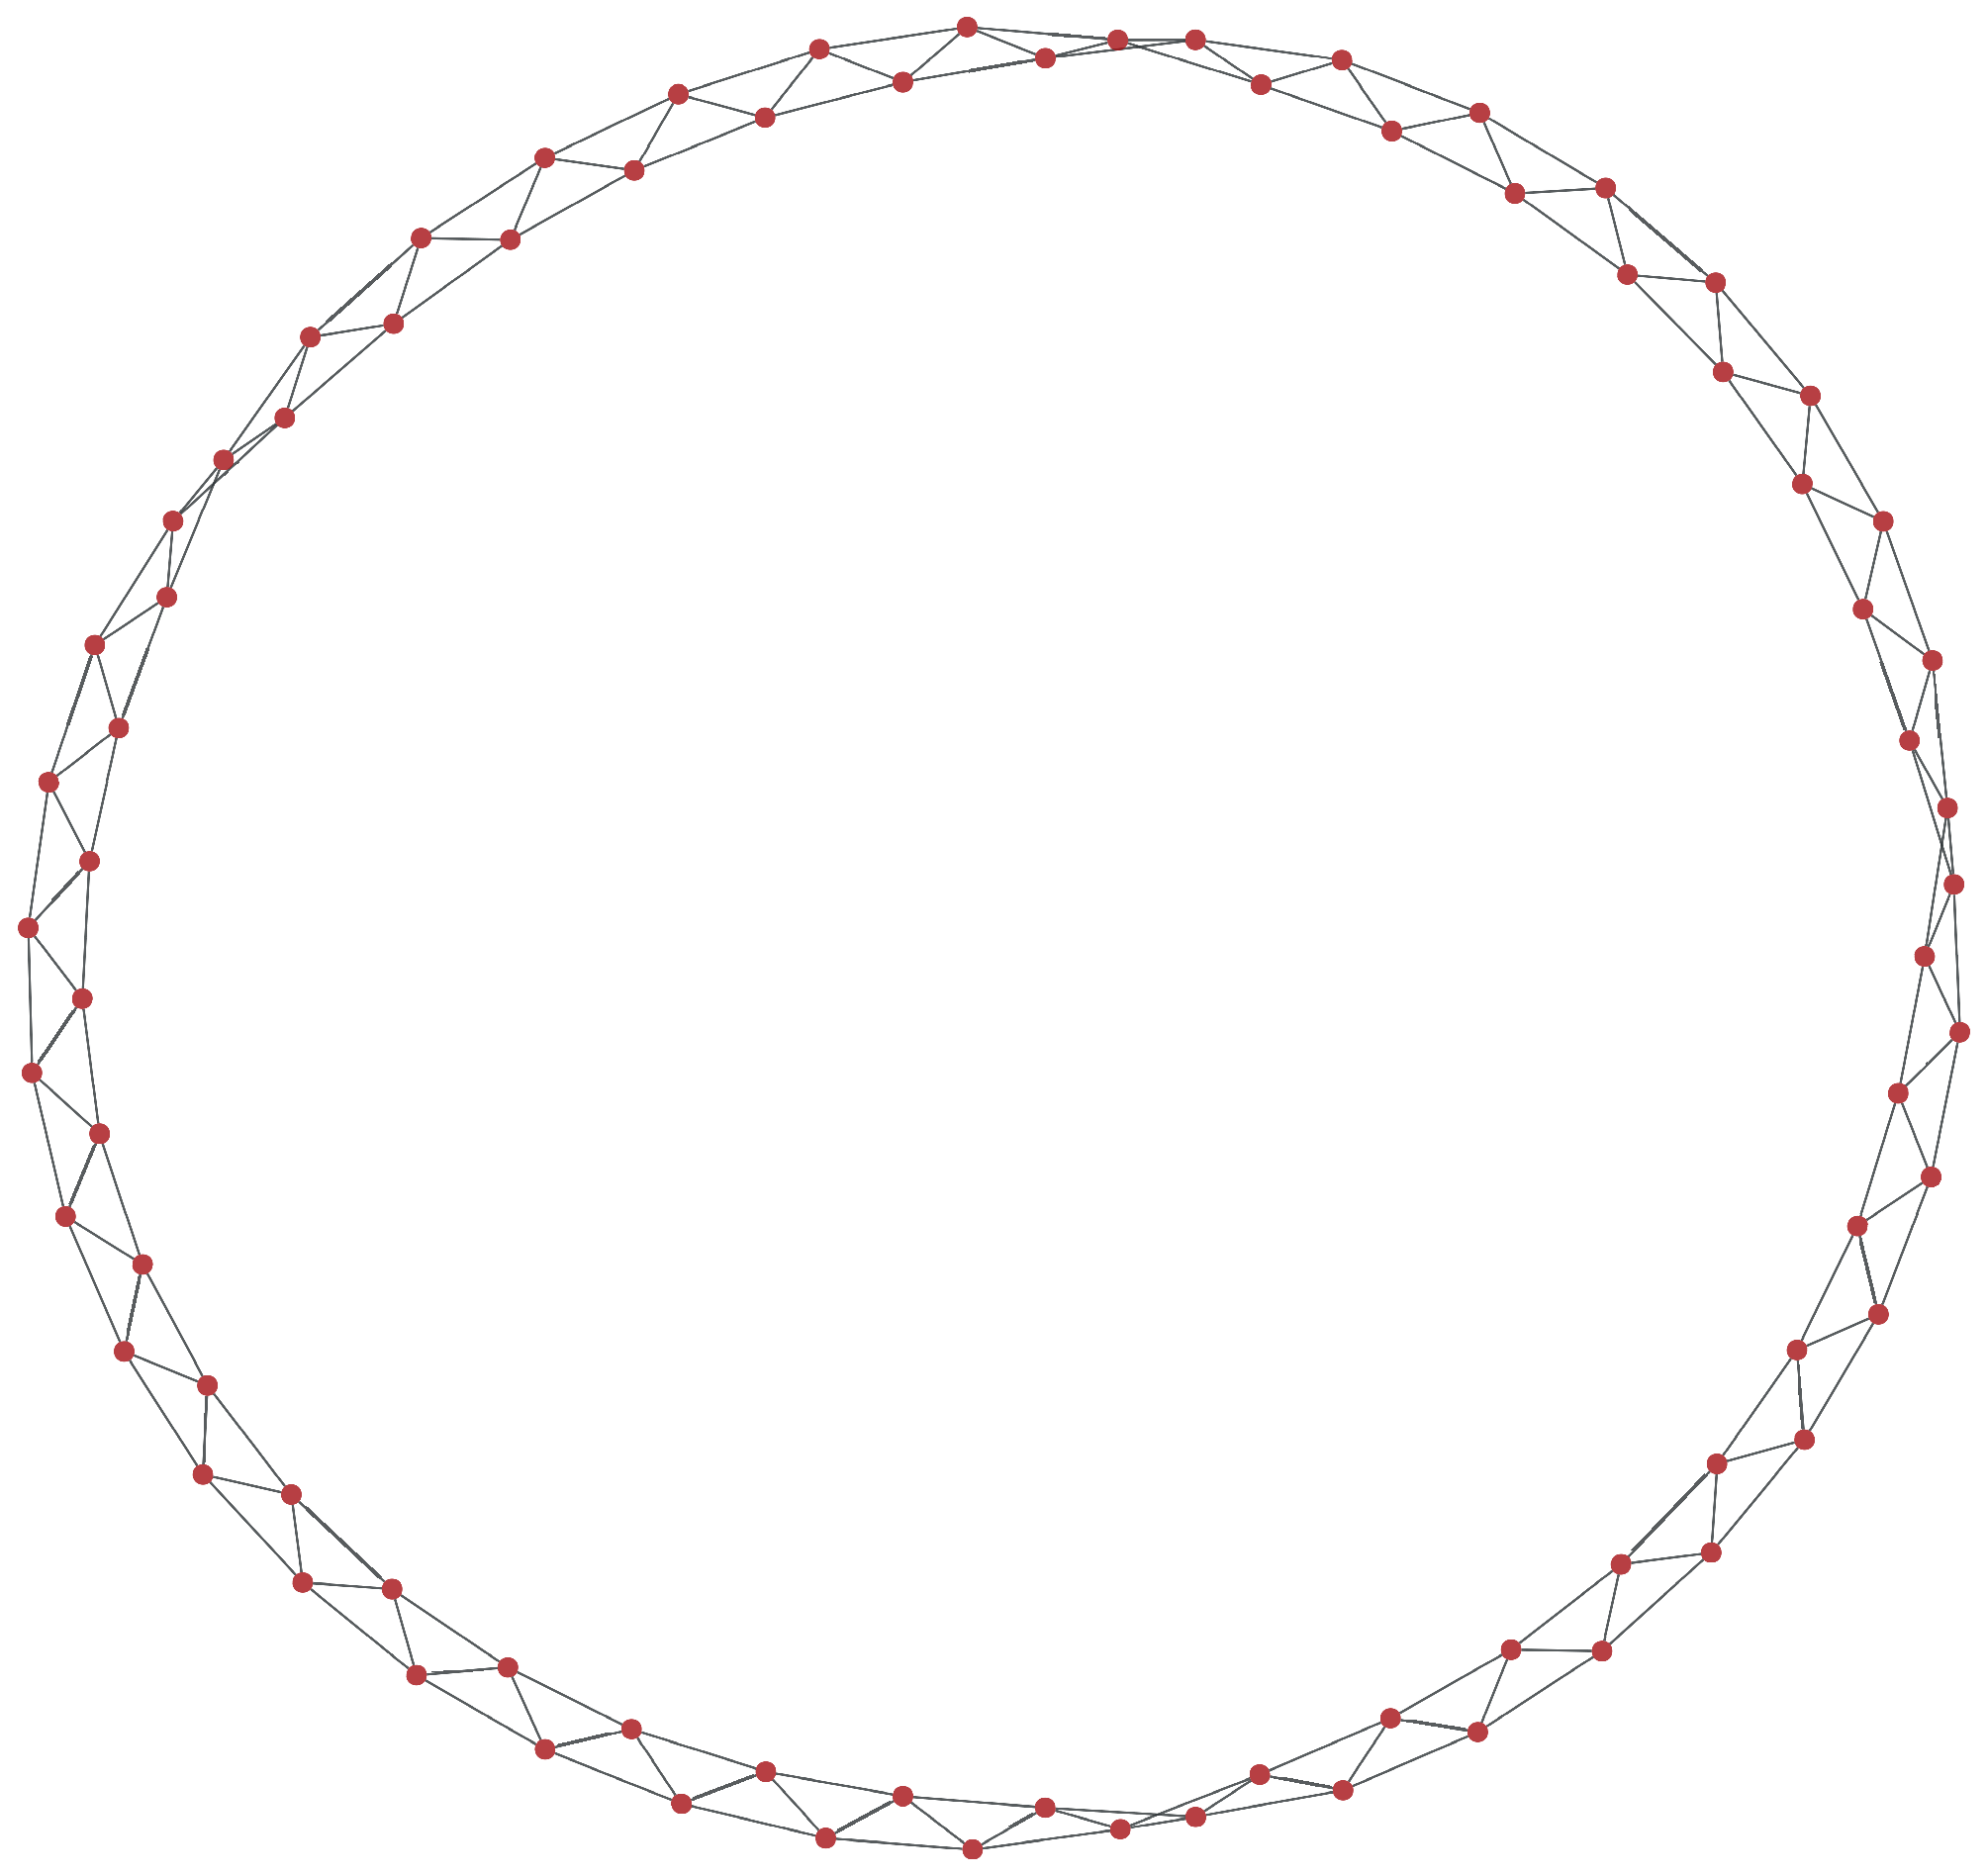
\includegraphics[width=0.4\textwidth]{./Immagini/Teoria/zoomring}
	\caption[Reticolo ciclico.]{Il punto di partenza del modello Watts-Strogatz: un reticolo con condizioni al contorno cicliche.}
	\label{fig:ring}
\end{figure}

Successivamente si procede a riarrangiare in maniera random i link tra i nodi, con una probabilità $p$ per ogni link di venire modificato. In questo modo si hanno un certo numero di link (in media $pnN$) che invece di essere tra nodi in prossimità, saranno tra nodi più lontani, come in Figura \ref{fig:watts}.

\begin{figure}[hb!]
	\centering
	\subfloat[$p = 0$]
	{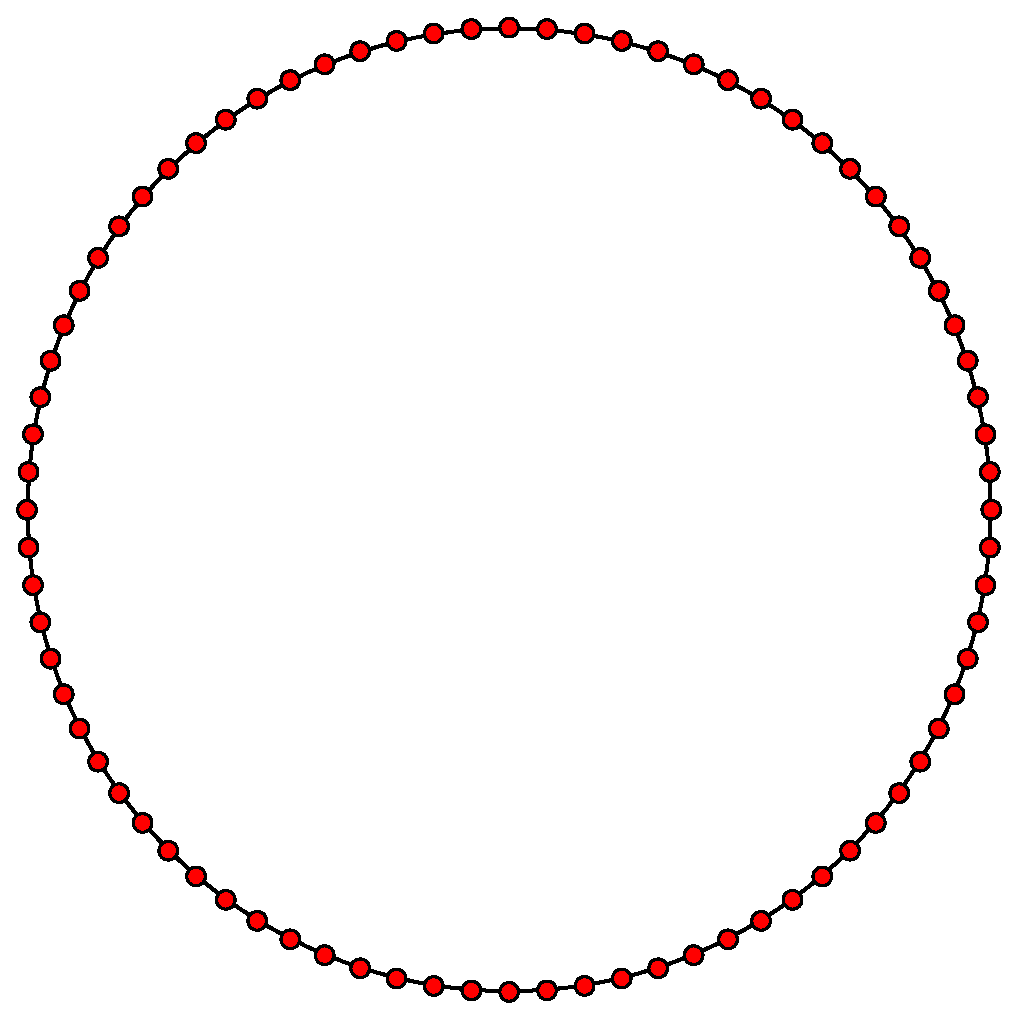
\includegraphics[width=0.3\textwidth]{./Immagini/Teoria/ringnet}}
	$\;\;$
	\subfloat[$p = 0.03$]
	{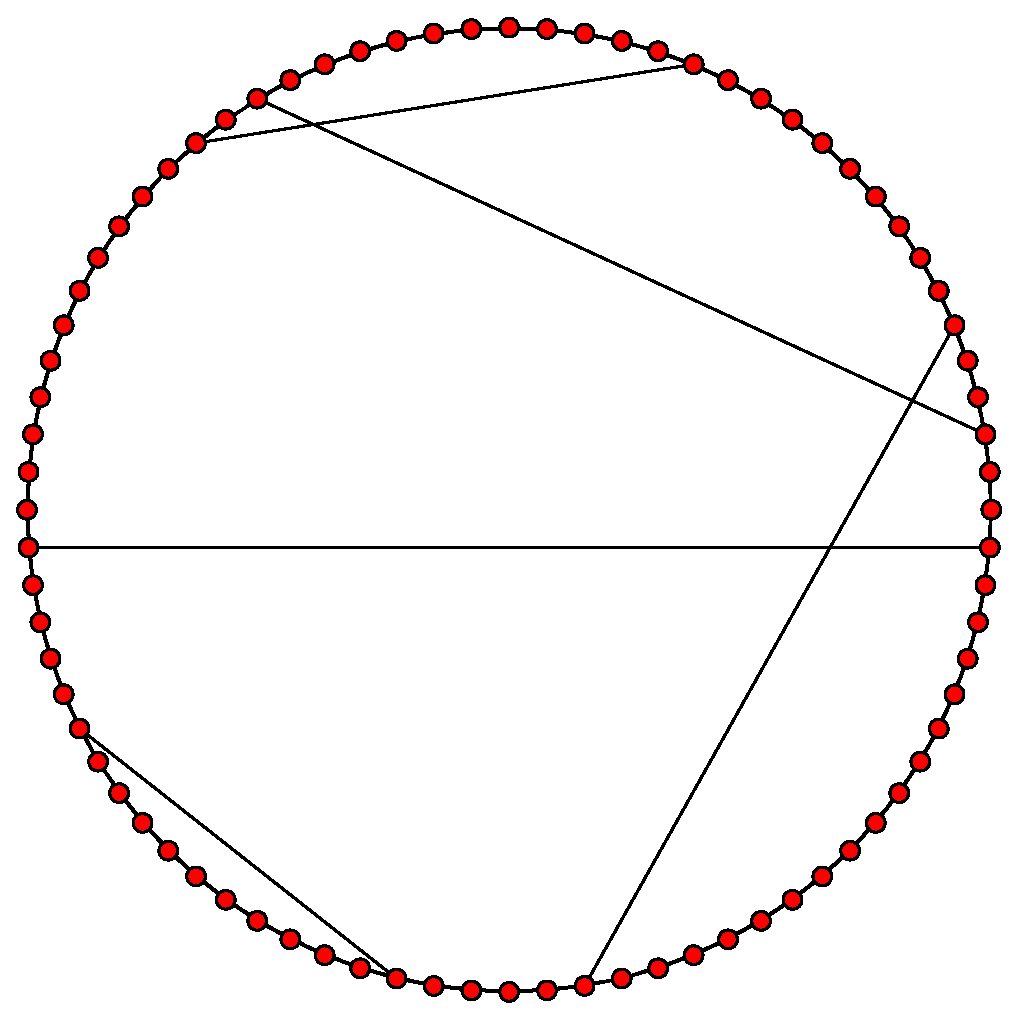
\includegraphics[width=0.3\textwidth]{./Immagini/Teoria/smallworld}}
	\\
	\subfloat[$p = 0.3$]
	{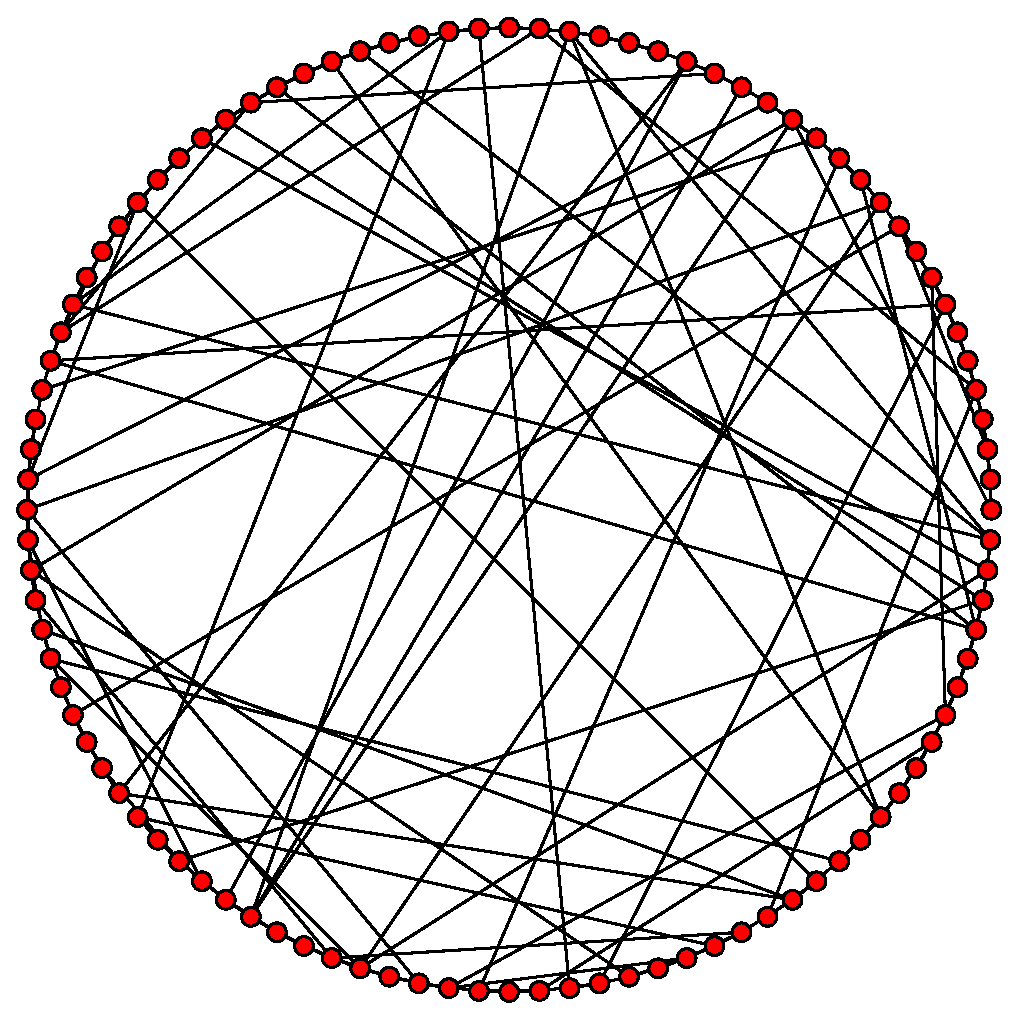
\includegraphics[width=0.3\textwidth]{./Immagini/Teoria/random-smallworld1}}
	$\;\;$
	\subfloat[$p = 1$]
	{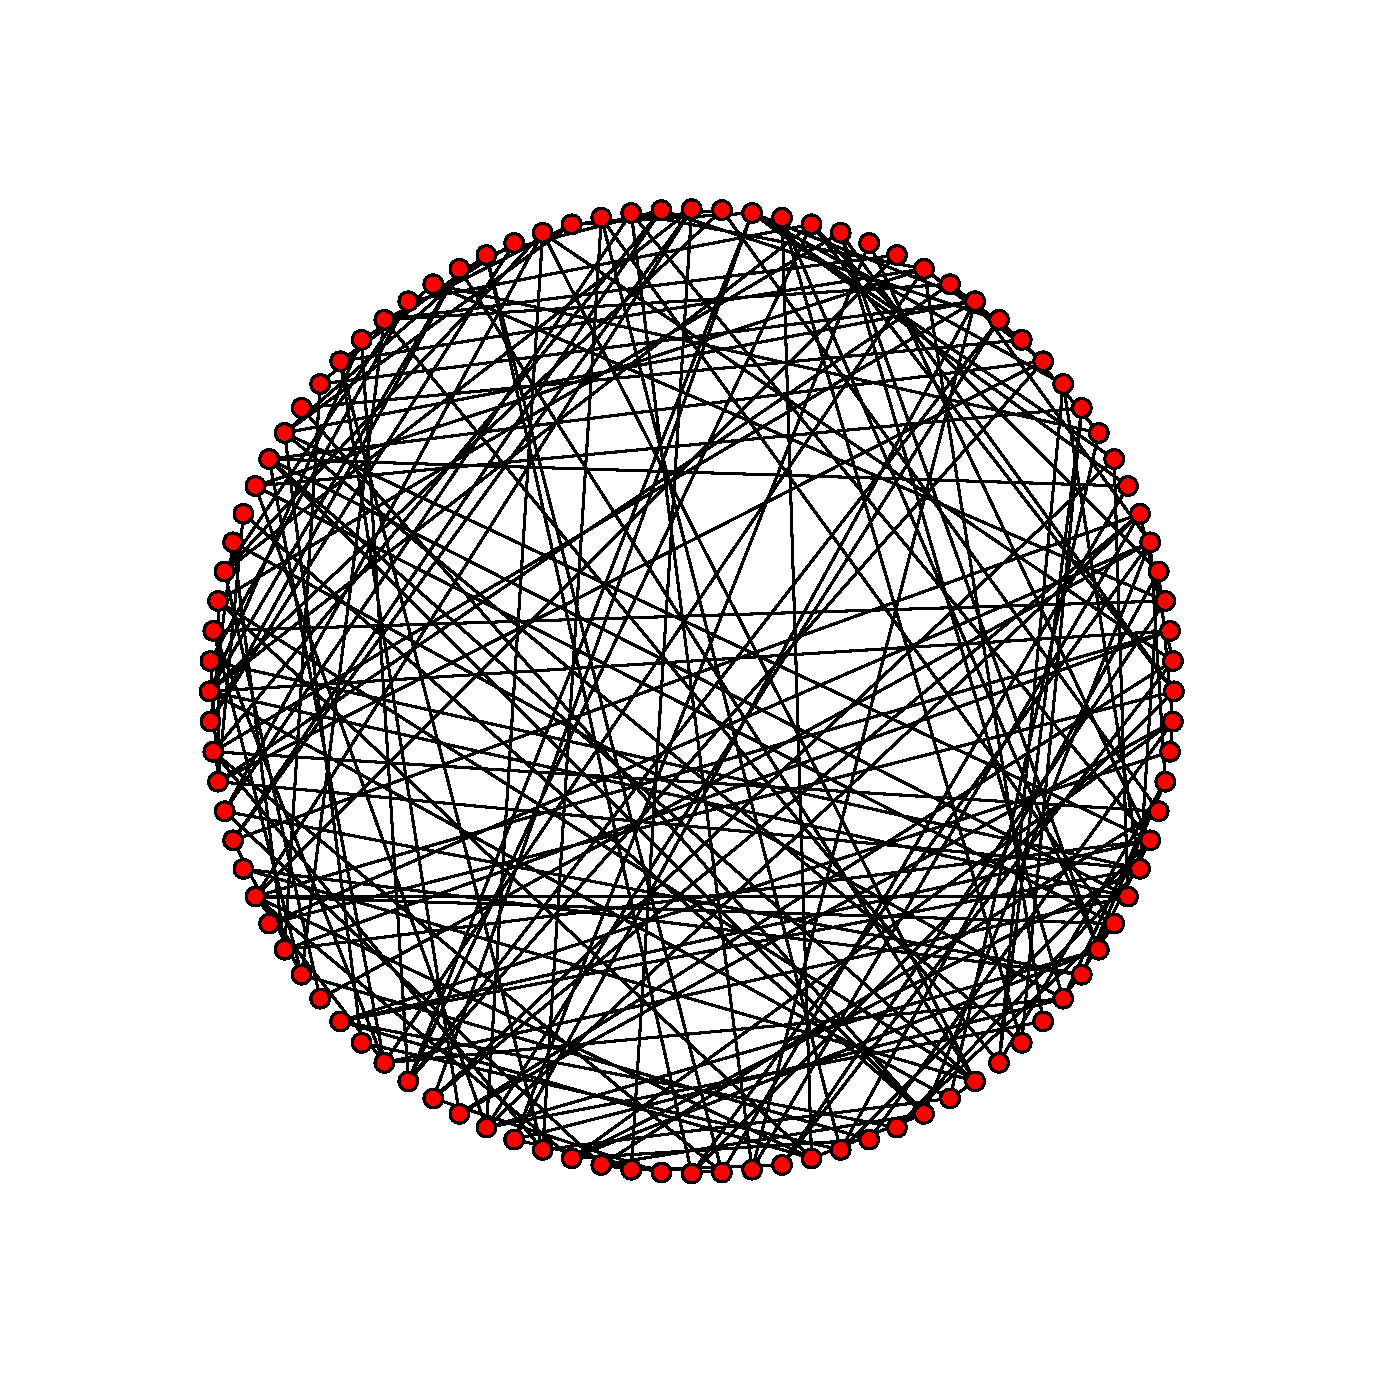
\includegraphics[width=0.3\textwidth]{./Immagini/Teoria/totalrandomwatts}}
	\caption[Generazione con modello Watts-Strogatz.]{Generazione di grafi con il modello Watts-Strogatz a differenti $p$ di rewiring.}
	\label{fig:watts}
\end{figure}
\clearpage
Con questo metodo, a seguito del \emph{rewiring} si ha il rischio che il grafo non sia più connesso. Ponendo $n>1$ ciò può essere evitato, portando la probabilità di avere un grafo non connesso quasi a zero già con $n=2$.
Con $p \rightarrow 1$ il grafo diventa simile a quello di una rete di Erdős-Renyi (v. Figura \ref{fig:confrontorandom}.

\begin{figure}[t!]
	\centering
	\subfloat[Grafo random]
	{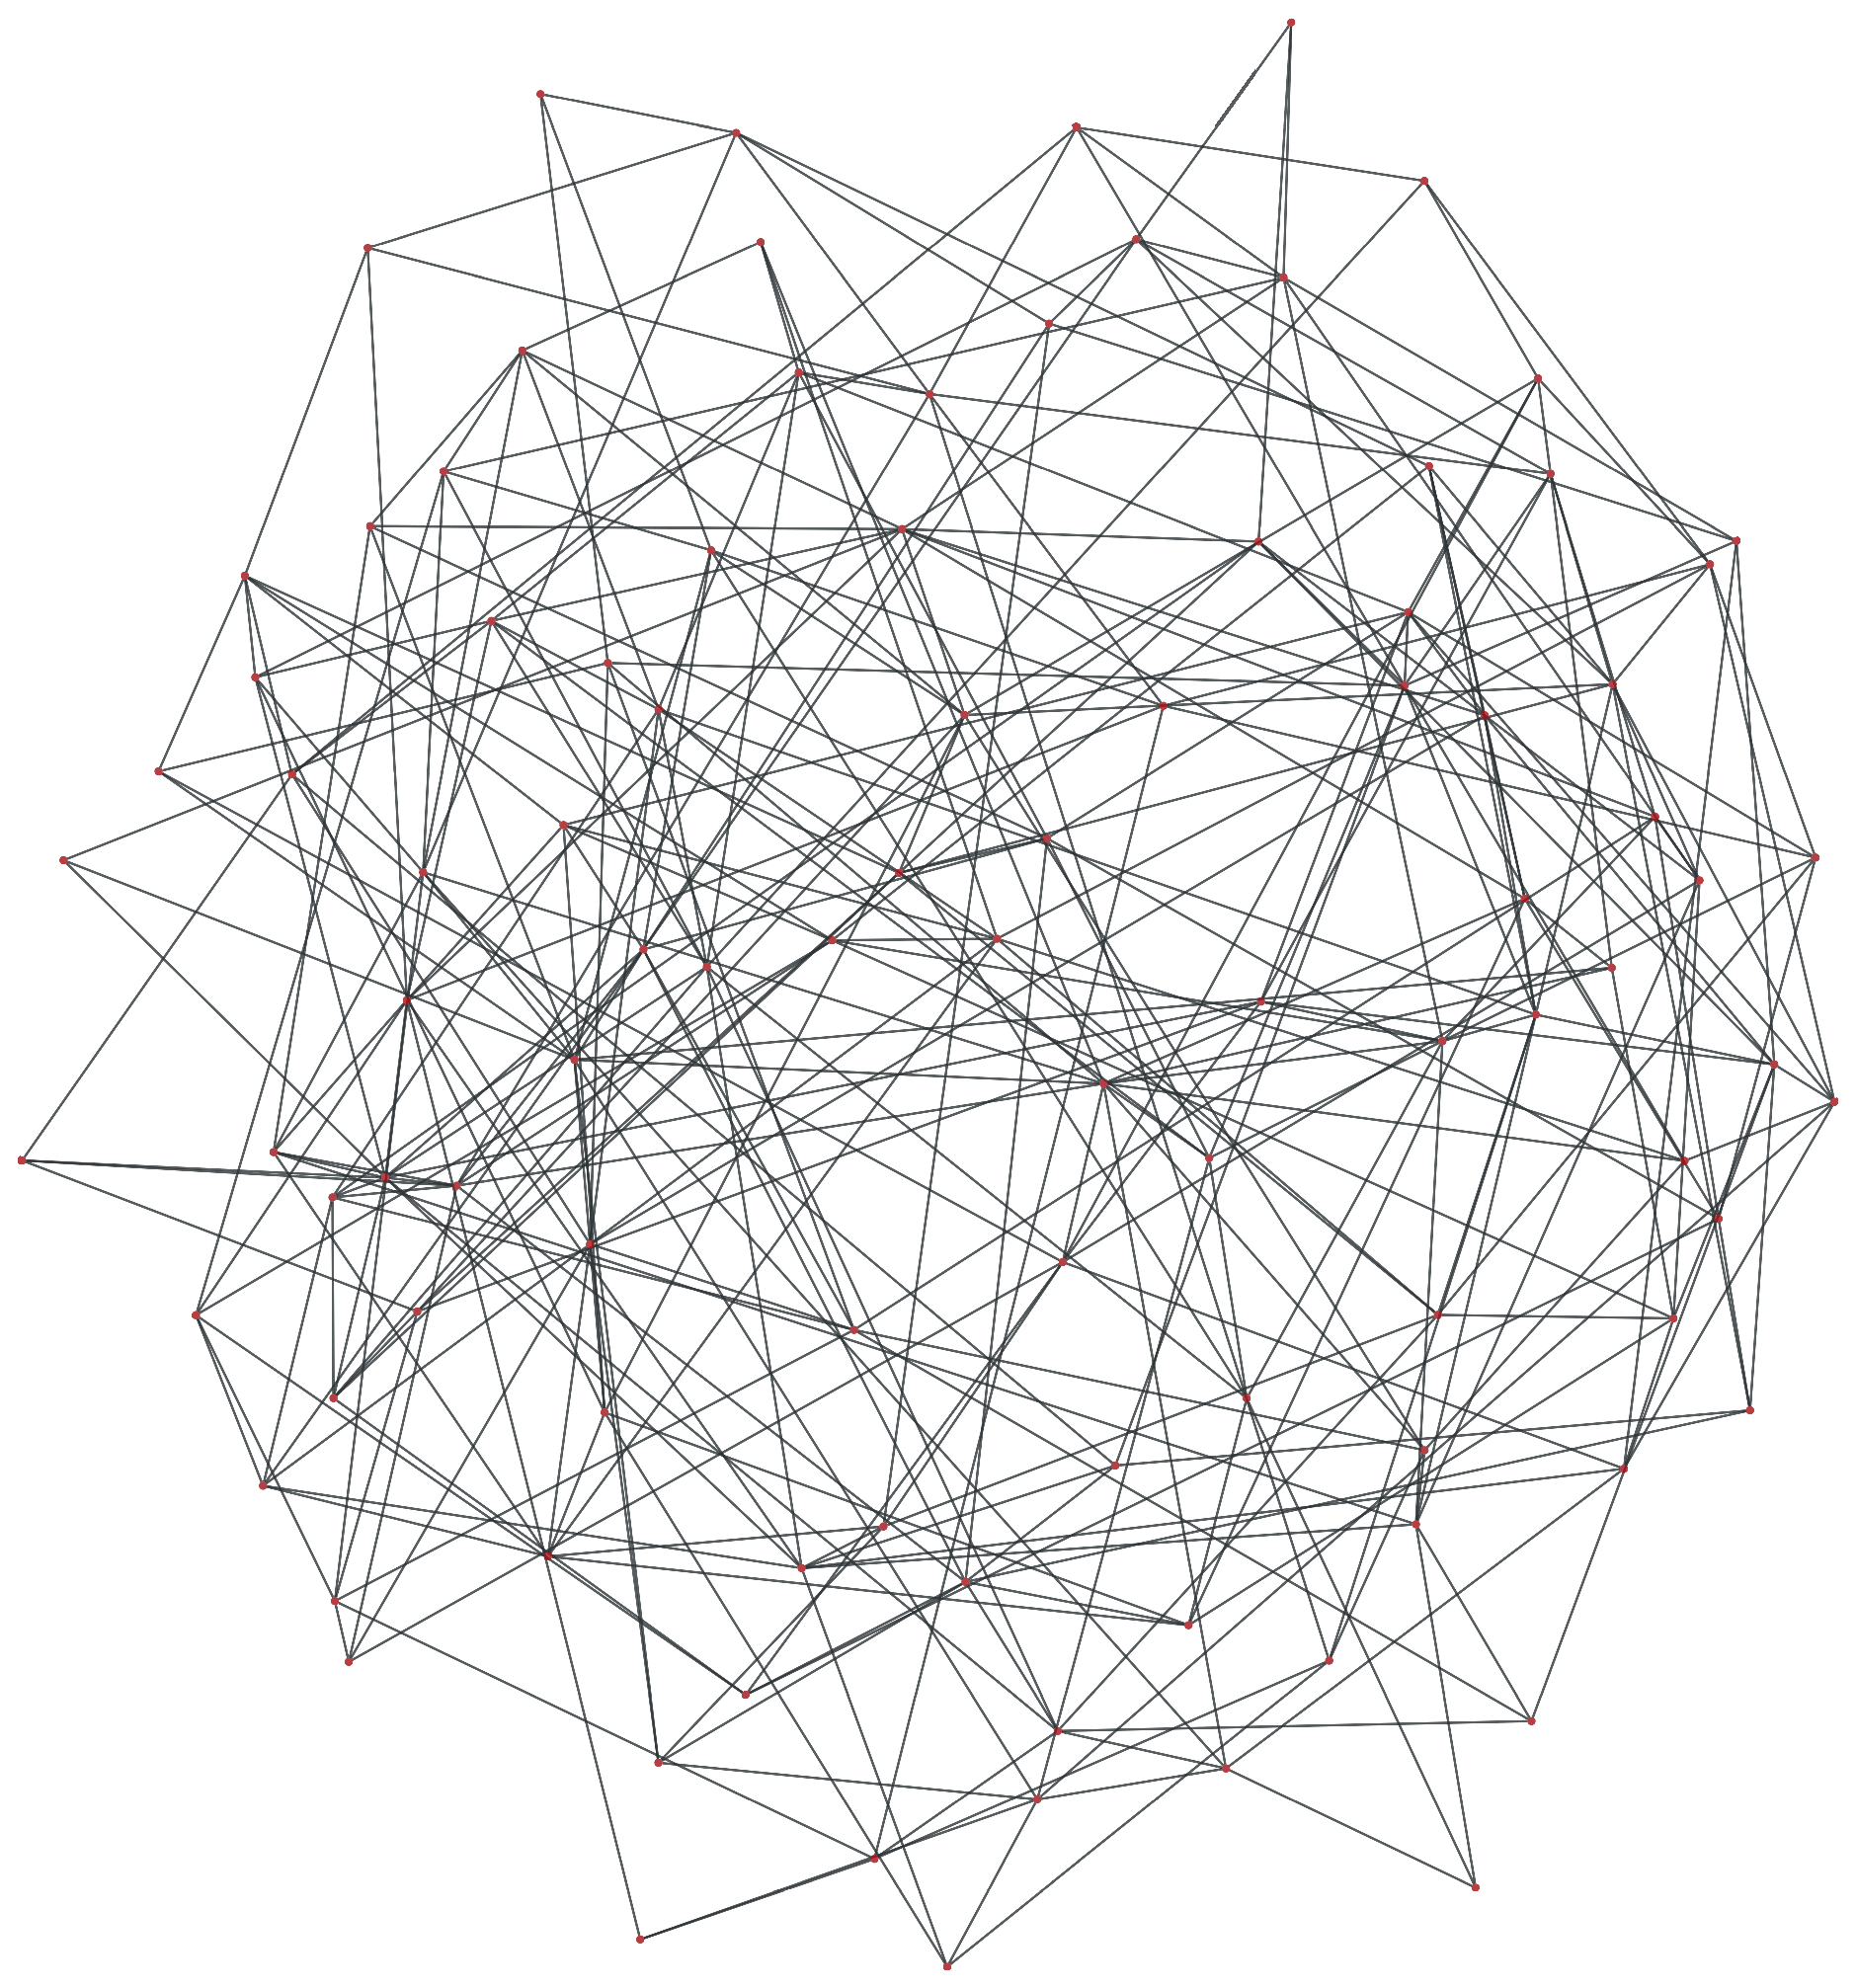
\includegraphics[width=0.3\textwidth]{./Immagini/Teoria/Erdosmodel}}
	$\;$
	\subfloat[Grafo small-world]
	{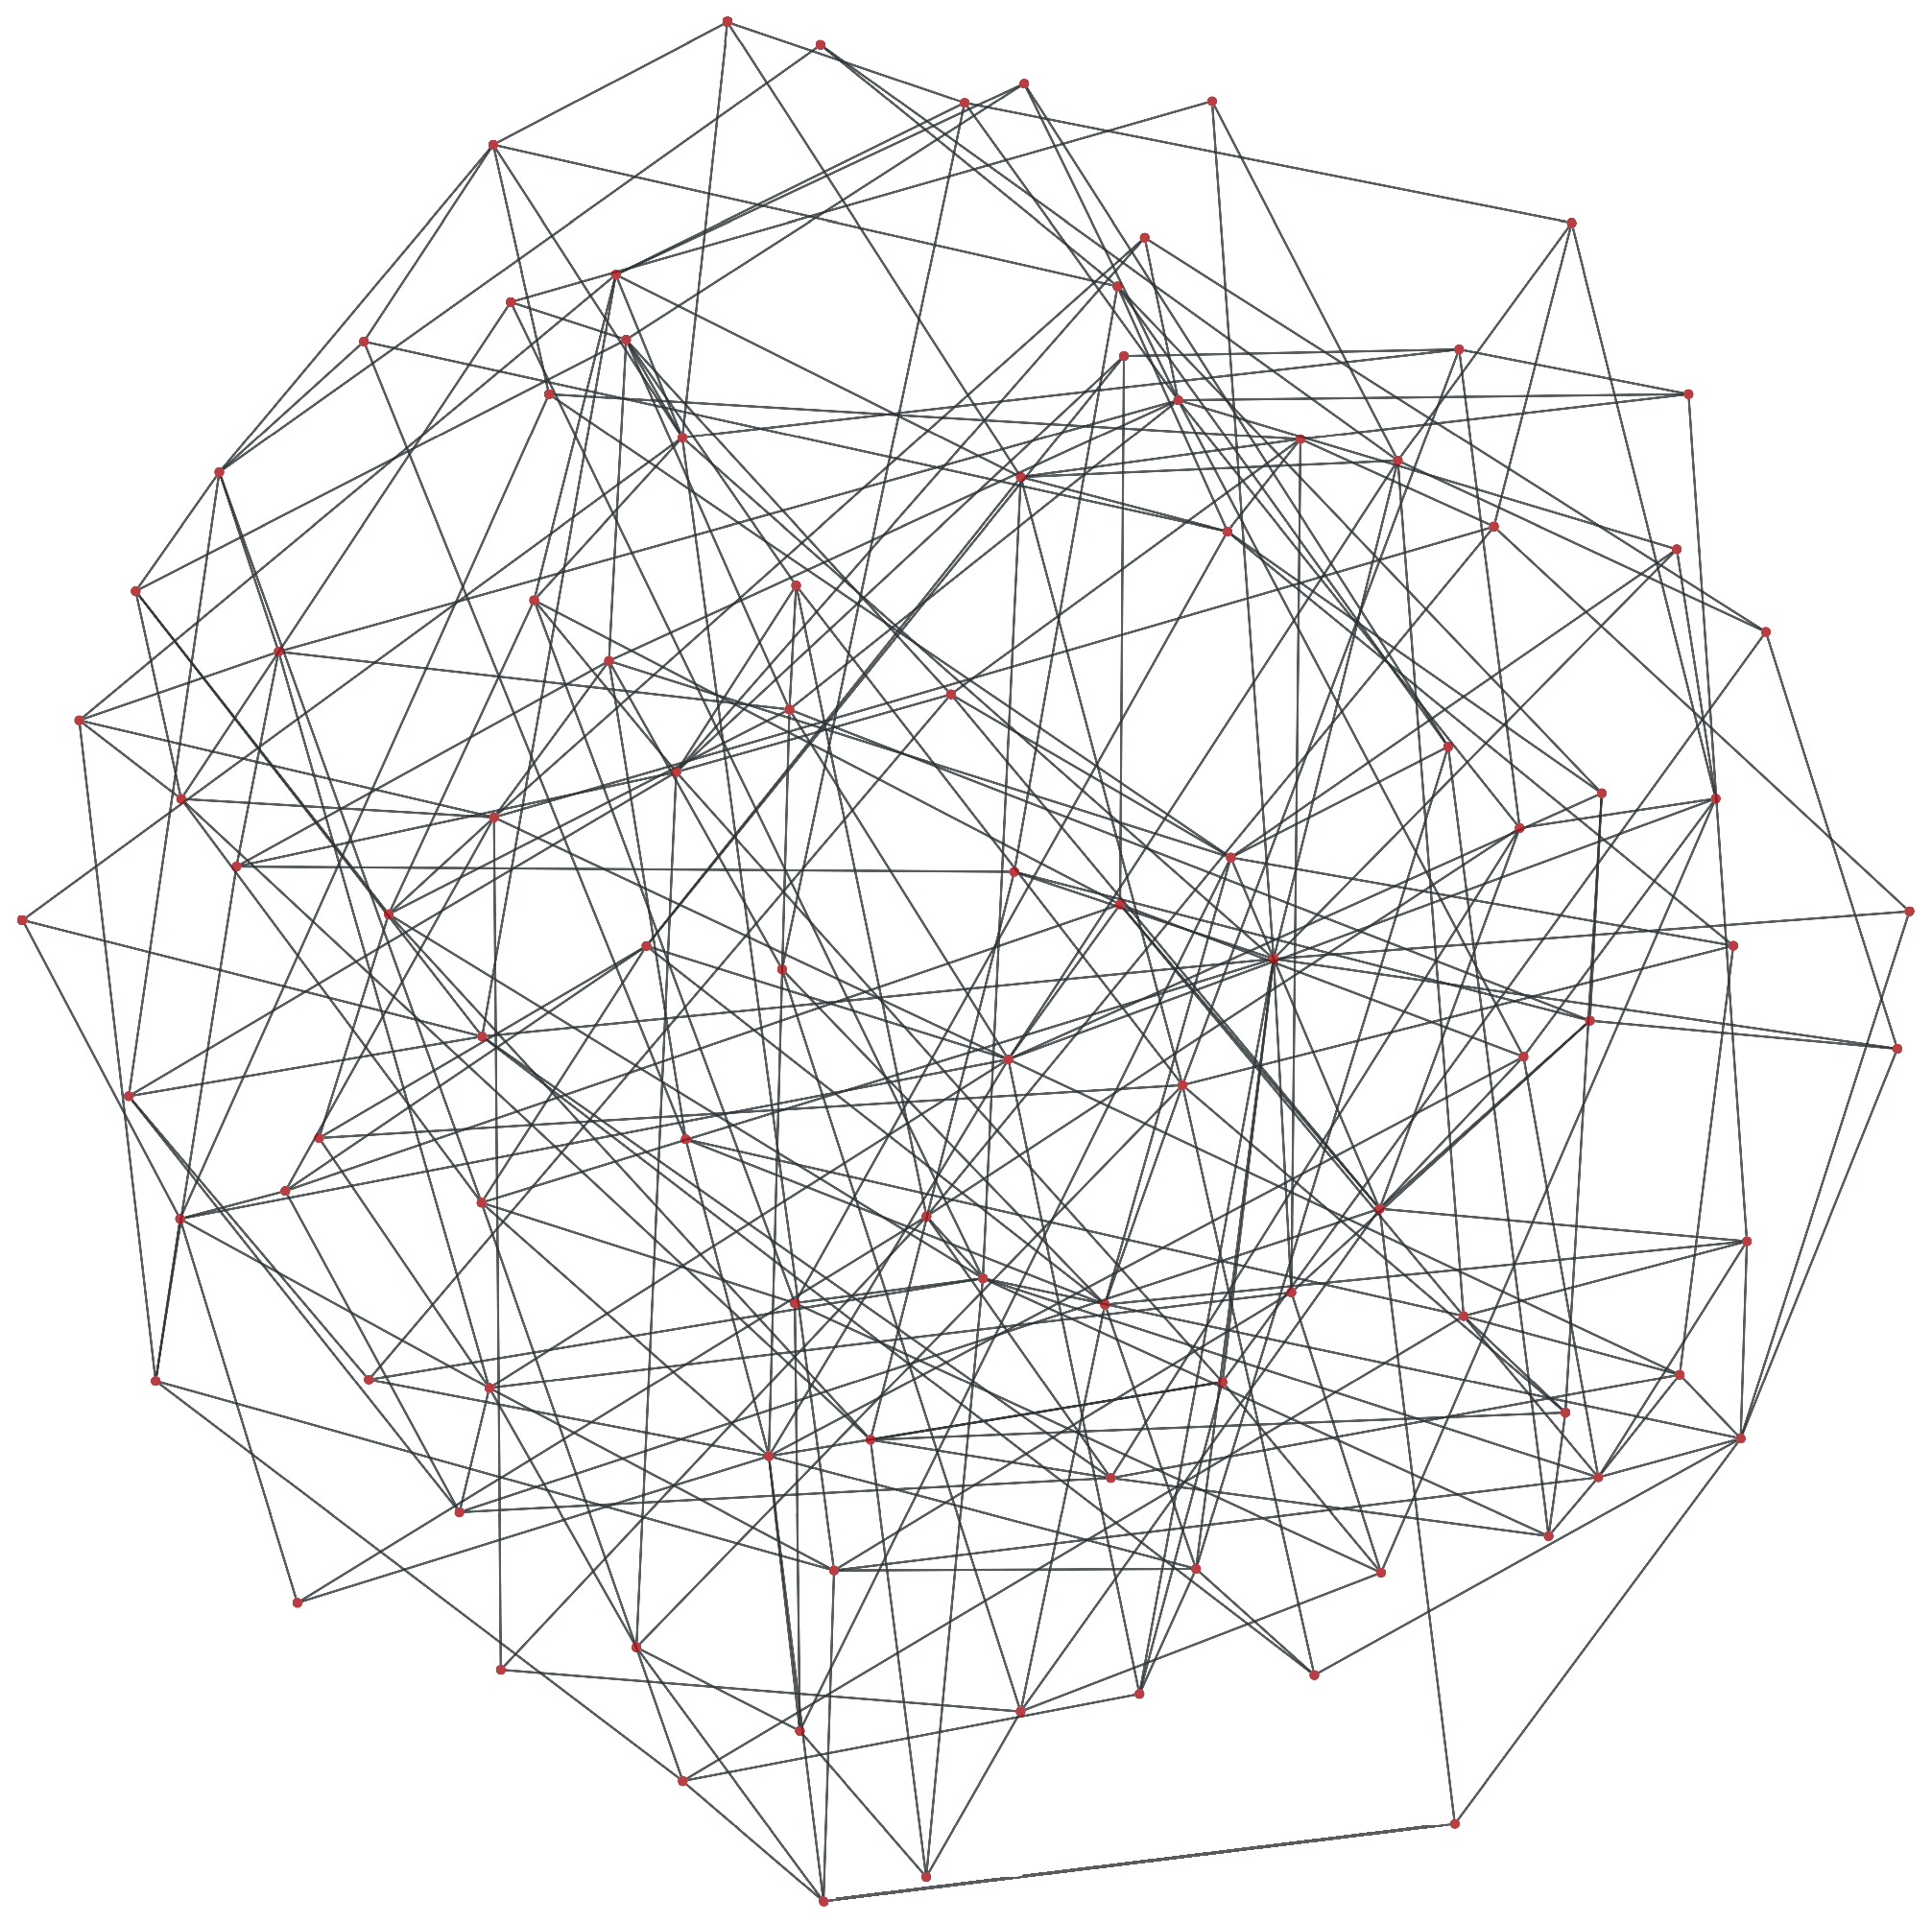
\includegraphics[width=0.3\textwidth]{./Immagini/Teoria/Wattsmodel}}
	\\
	\subfloat
	{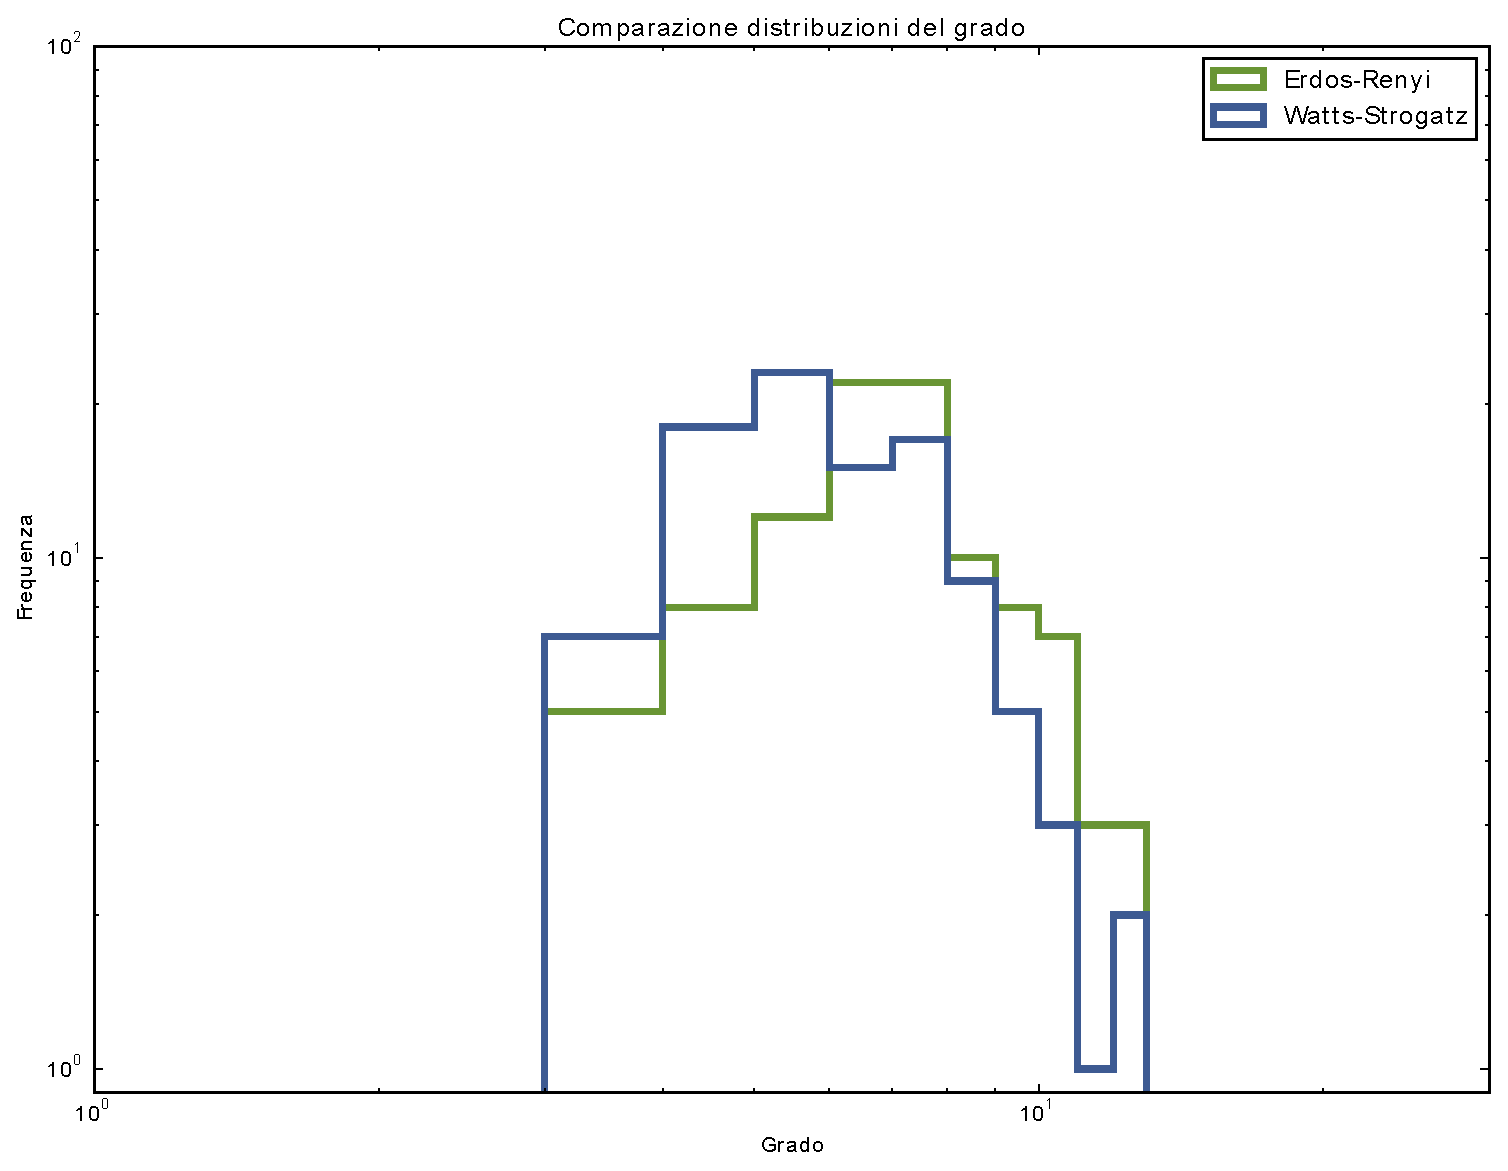
\includegraphics[width=0.8\textwidth]{./Immagini/Teoria/ComparGradeModel}}
	\caption[Confronto grafi random.]{Confronto tra due grafi da 100 nodi: uno generato con il modello Erdos-Renyi ($p=7\%$) e uno con il modello Watts-Strogatz partendo da un reticolo con nodi connessi ai primi 3 vicini e il 100\% di probabilit\`a di rewiring. A parte la somiglianza dei grafi, le distribuzioni del grado hanno simile comportamento.}
	\label{fig:confrontorandom}
\end{figure}

Per avere una rete tipica che abbia un numero di connessioni non troppo elevato, ma non così poco da rischiare da avere un grafo non connesso a seguito dell'operazione di rewiring, possono essere considerati degli $N$ e $n$ tali che $N>>n>>ln(N)>>1$. Con queste condizioni la distribuzione del grado $P(k)$ ha una forma gaussiana la cui media coincide con $n$, con $\sigma$ più piccole per $p$ basse, tendente a una delta di Dirac per $p \rightarrow 0$. 

Infatti, mentre con $p=0$ si ha un reticolo con grado uguale per ogni nodo, l'operazione random di rewiring introduce una casualità sulla $P(K)$ ben descritta da una gaussiana per $N$ grandi, che però ha una larghezza sensibilmente inferiore a quella di una rete random, portando a una rete ancora più omogenea.  

Valori tipici di $\langle l \rangle$ per le reti reali sono ben descritti dal modello di Erdős e Renyi secondo l'equazione \ref{eq:lunghezze} \parencite{Barbalbert2002}, cioè ci si aspetta scali in modo logaritmico fissato $\langle k \rangle$. In una rete generata secondo il modello di Watts-Strogatz le lunghezze dei cammini, fissato $n \equiv \langle k \rangle$, scalano in media in modo diverso al variare di $p$. Per $p$ molto basse ($p << 1/nN$) le lunghezze caratteristiche sono proporzionali alla dimensione del grafo, il quale è ancora molto simile a una reticolo; abbastanza presto, per $p >> 1/nN$, \footnote{$p >> 10^{-4}$ per una rete con $10^3$ nodi e $P(k)$ centrata in 10} vi è invece un largo intervallo di $p$ che vede già verificarsi il fenomeno small-world, con le lunghezze dei cammini che scalano come $ln(N)$ in accordo con le reti reali.  

L'altra caratteristica fondamentale di uno small-world è che abbia un clustering abbastanza alto in relazione a una rete puramente random. Per $p = 0$ il reticolo ha un $C(0)$ costante al variare di $N$; all'aumentare di $p$, presa una tripletta chiusa, la probabilità che tutti e tre i link rimangano inalterati è $(1-p)^3$  e i suoi due primi vicini hanno probabilità $p^3$ di vedere almeno uno dei loro link riarrangiato. Dato che $C=N_\triangle/N_\wedge$ e che $N_\wedge$ rimane costante con il rewiring, si può porre 
\[C(p) \propto N_\triangle (p) \Rightarrow C(p) \sim C(0)(1-p)^3, \]
con $C(0) \sim 0.75$ per $N$ grande. Ricordando che per il modello di Erdős-Renyi $C_{ER}=p$, e che per modellizzare una rete reale $p$ solitamente è abbastanza piccola dato che $\langle k \rangle = Np$, risulta che per valori di $p \lesssim 0.25$ si hanno velocemente $C_{WS}$ sensibilmente maggiori di $C_{ER}$ (v. Figura \ref{fig:confrontoC}.

\begin{figure}[t!]
	\centering
	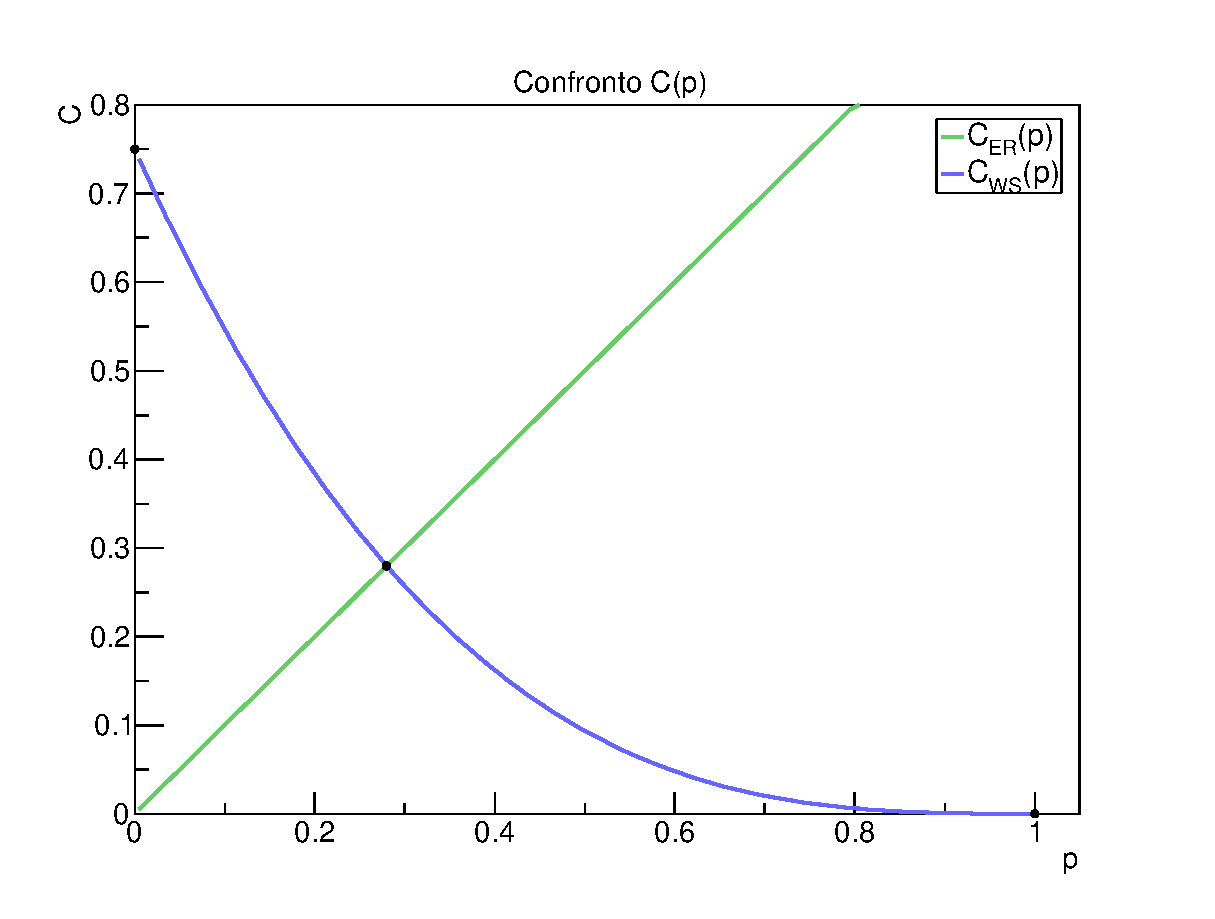
\includegraphics[width=0.6\textwidth]{./Immagini/Teoria/confrontoC}
	\caption[Confronto clustering.]{Confronto tra i coefficienti di clustering teorici dei due modelli, al variare del rispettivo parametro $p$.}
	\label{fig:confrontoC}
\end{figure}

Concludendo, un grafo è considerato small-world se ha contemporaneamente piccole distanze medie e, a differenza dei grafi random,  una clusterizzazione relativamente elevata. Pertanto il modello di Watts e Strogatz descrive in maniera soddisfacente reti che abbiano queste caratteristiche, purché non siano scale-free.

\subsubsection{Barabasi-Albert} 
Molte importanti reti reali di grandi dimensioni hanno la notevole caratteristica di avere un certo livello di invarianza di scala. Questa è manifestata da una distribuzione del grado che segue una funzione a legge di potenza $P(k)\sim k^{-\gamma}$, con $\gamma$ compreso quasi sempre tra $2$ e $3$, in maniera sempre più esatta al crescere di $k$. Mentre le reti random possono riprodurre una $P(k)$ arbitrario, e quindi anche una \emph{power-law}, ma non riescono a generare grafi connessi e con $\langle l \rangle$ non definibile \parencite{Barbalbert2002}, le reti small-world riproducono bene le proprietà di clustering e cammini medi, ma non possono portare a $P(k)$ power-law. Serve pertanto un modello che riproduca piccoli diametri, grandi clustering e $P(k)$ a legge di potenza.

%TODO final decomment
\begin{figure}[t!]
	\centering
	\includegraphics[width=0.9\textwidth]{./Immagini/Teoria/Barabalbert1}
	\caption[Albero scale-free]{Esempio di grafo generato con il modello di Barabasi-Albert. Con $m=1$ \`e evidente la struttura frattale, ma essendo un grafo ad albero il clustering \`e nullo.}
	\label{fig:barabalbero}
\end{figure}

I modelli di Erdős-Renyi e Watts-Strogatz partono da una configurazione di nodi e poi distribuiscono o riarrangiano i link con una certa probabilità \emph{uniforme} per tutti i link. Le reti reali, tuttavia, spesso partono da un certo numero piccolo di nodi e successivamente crescono. Il primo punto chiave del modello formulato da Barabasi e Albert è proprio il concetto di crescita: la rete parte a $t=0$ con $m_0$ nodi e a ogni step temporale si aggiunge alla rete un nodo con un certo numero $m < m_0$ di link da assegnare agli altri nodi esistenti. Il secondo riguarda il fatto che la probabilità di \emph{attachment} di un nuovo nodo agli altri non è uniforme su tutti i nodi ma preferenziale: il \emph{preferential attachment} dà quindi una maggiore probabilità $\Pi (k_i)$ di collegamento di un nodo nuovo a un certo nodo $i$ in maniera proporzionale al suo grado, secondo la formula
\[\Pi (k_i) = \frac{k_i}{\sum_j k_j}.\]

La costruzione della rete avviene in modo dinamico, pertanto il grado di un nodo $i$ sarà funzione crescente del suo tempo di vita nella rete, con una probabilità di attachment dei nuovi nodi a $i$ anch'essa dipendente da $t$. Pertanto, con l'andare del tempo il grado di $i$ aumenterà sempre più velocemente. Approssimando $k_i$ a una variabile continua per $t$ grandi, dato che 
\[\frac{dk_i}{dt} = m \Pi (k_i) = m \frac{k_i}{\sum_{j=1}^{N-1} k_j} = m \frac{k_i}{2mt - m} = \frac{k_i}{2t - 1} \sim \frac{k_i}{2t},\]
dove $m$ è il numero di link aggiunti per iterazione, ponendo quindi la condizione iniziale per il nodo $i$, $k_i(t_i) = m$
\[ \Rightarrow k_i(t) = m \left(\frac{t}{t_i}\right)^\frac{1}{2}. \]

Ovviamente se il grado di un nodo è funzione di $t$, anche la P(k) lo sarà. Definendo $P(k_i(t)<k)$ la probabilità che un nodo $i$ abbia un grado minore di un certo valore $k$, la distribuzione del grado $P(k)$ può essere derivata ponendola uguale a $dP(k_i(t)<k)/dk$, ottenendo per $t\rightarrow \infty$:
\[ P(k)\sim 2m^2 k^{-3}. \]


Il modello di Barabasi e Albert è un modello minimale, importantissimo perché il primo in grado di riprodurre un grafo che mostrasse un'invarianza di scala, ma che in alcuni aspetti mal si accorda con quelle reti reali con caratteristiche scale-free. Per cominciare la distribuzione del grado è una legge di potenza con esponente $3$,ma le reti scale-free solitamente hanno un esponente inferiore, seppur maggiore di $2$. Benché non sia possibile calcolare in modo analitico $\braket{l}$ e $C$ per una rete di Barabasi-Albert, da simulazioni numeriche è possibile ottenerne quantità caratteristiche. 

Il cammino medio risulta sottostimato rispetto alle reti reali e il coefficiente di clustering non è costante con l'aumentare di $N$ come per le reti reali ma diminuisce, anche se più lentamente di una rete random\footnote{Ovviamente il coefficiente di clustering dipende dal numero $m$ di link generati per ogni nuovo nodo. Con $m = 1$ il clustering \`e nullo dato che il grafo \`e un albero, mentre $C \neq 0$ per $m>1$ e cresce all'aumentare di $m$, mantenendosi comunque al di sotto dei valori di reti reali con parametri simili.} \parencite{Barbalbert2002}. Per questo motivo il modello iniziale è stato integrato e reso più complesso.  

\begin{figure}[ht!]
	\centering
	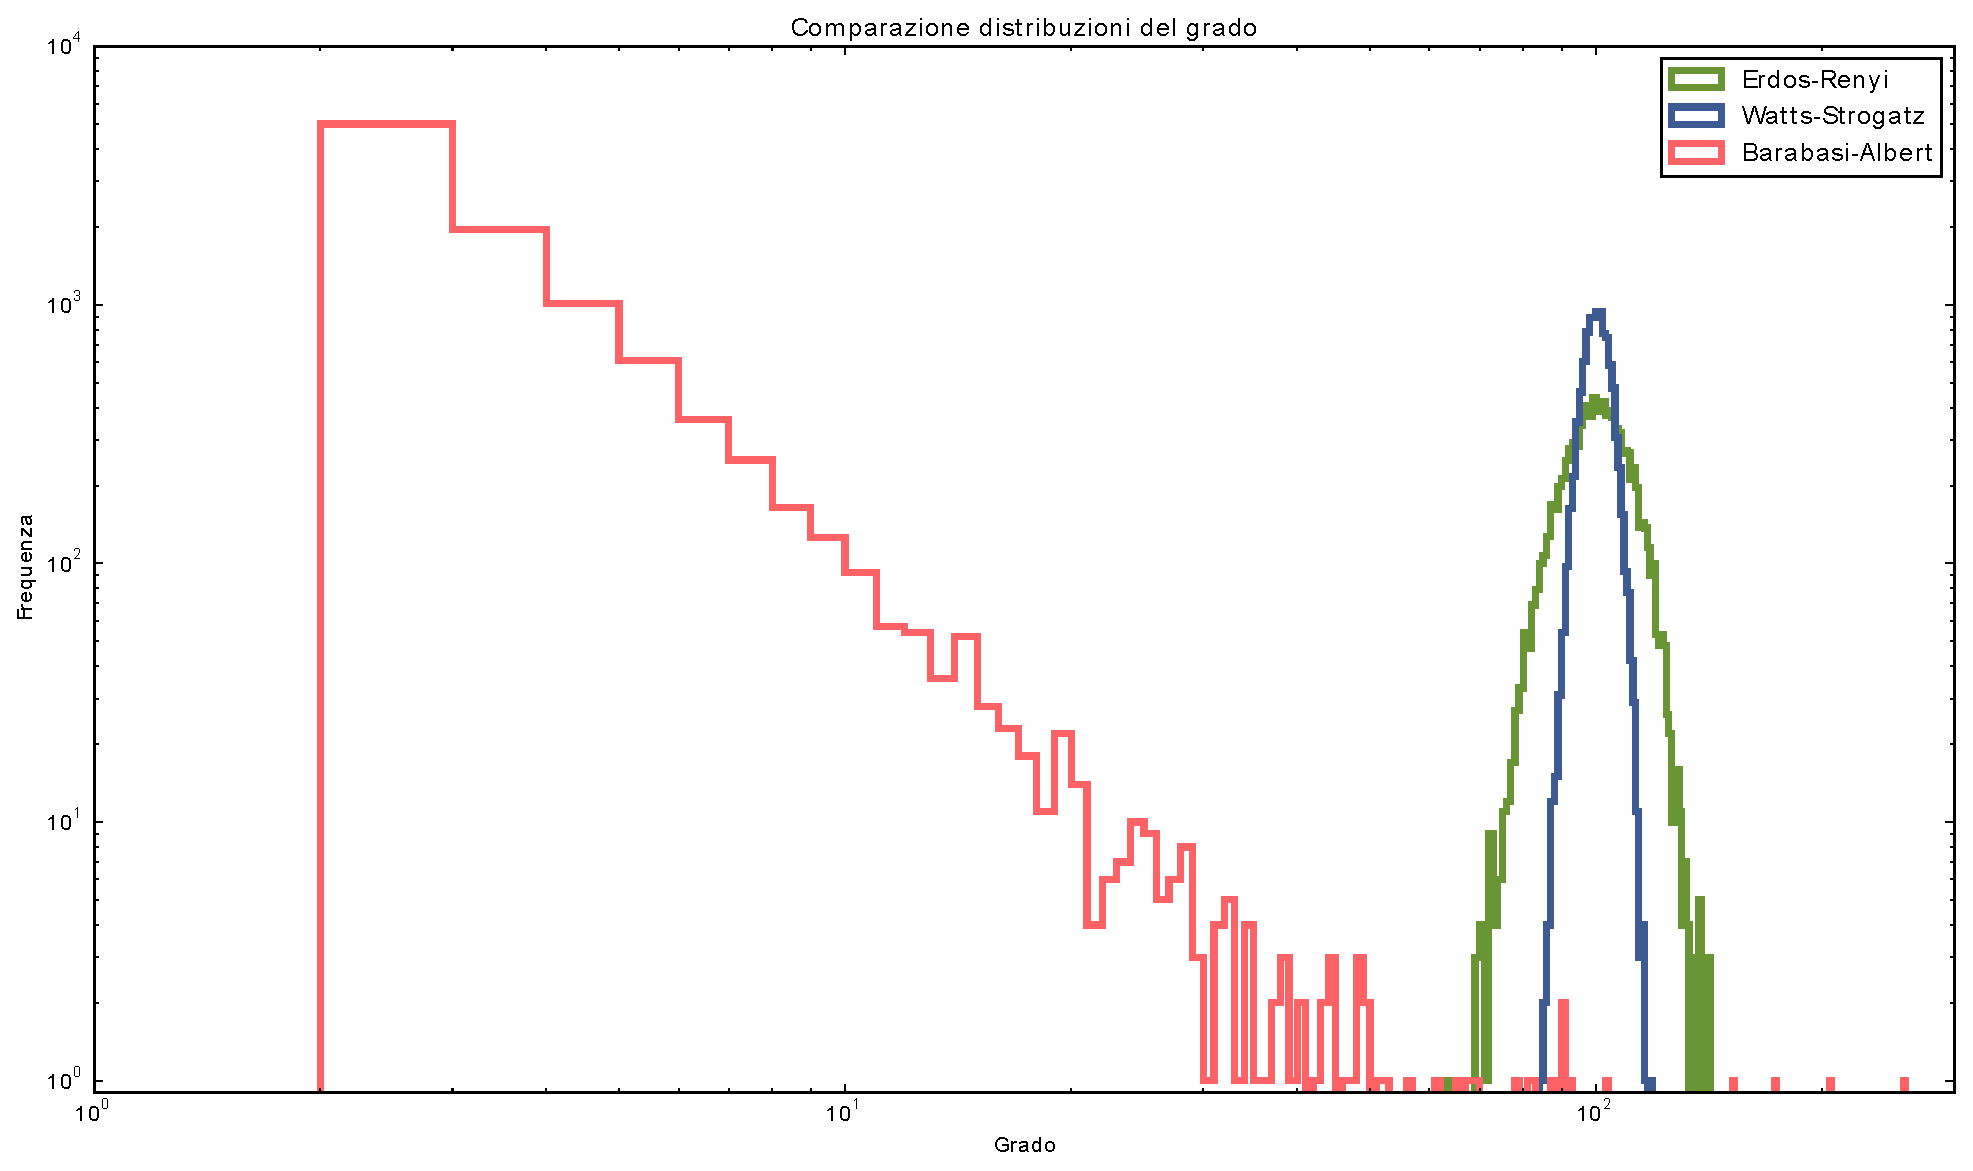
\includegraphics[width=0.9\textwidth]{./Immagini/Teoria/compareSameN}
	\caption[Confronto $P(k)$]{Confronto tra le distribuzioni del grado dei tre modelli esposti.}
	\label{fig:confrontoGradi}
\end{figure}

\clearpage
\section{Teoria della percolazione}
\label{sec:percola}
Per percolazione, in analogia con i liquidi, si intende il passaggio di informazione da un lato all'altro di una rete. Nello specifico, quando si fa uno studio percolativo di una rete, si cerca l'esistenza o meno di un cluster che ricopra l'intera rete (\emph{spanning cluster}, o \emph{giant cluster}). Il giant cluster \`e definito come quella componente di una rete le cui dimensioni sono dello stesso ordine della dimensione della rete complessiva (e quindi gli altri nodi o cluster minori hanno dimensioni di ordini inferiore), cio\`e il rapporto tra le sue dimensioni e le dimensioni dell'intera rete \`e $\sim 1$.

Tipicamente uno studio percolativo su una rete random consiste nell'individuare, durante la costruzione della rete partendo da $N$ nodi scollegati, la soglia percolativa $p_c$, cio\`e la probabilit\`a di creazione link tale che compaia lo spanning cluster. Nel caso di una rete costruita con il modello di Barabasi-Albert la questione non si pone, dato che per definizione questa \`e composta da un solo cluster in crescita progressiva. Inoltre, dato che una rete di antenne cellulari nasce con una progettazione molto dettagliata in modo che venga costruita gi\`a oltre la soglia percolativa, nel caso in esame non \`e praticabile n\'e interessante individuare $p_c$ in costruzione. In questo caso ha pi\`u senso individuare la soglia percolativa per distruzione della rete. 

Uno studio per distruzione pu\`o avere pi\`u approcci che portano a soglie diverse:
\begin{itemize}
 \item se si parte da una rete con uno spanning cluster, rimuovendo link tra tutte le coppie di nodi connesse con una certa probabilit\`a, si avr\`a una $p_d$ oltre la quale la rete non percola pi\`u. In questo caso $p_{d_{link}} = 1-p$ soltanto se si parte da un grafo completamente connesso.
 %TODO BARBASI LO CHIAMA UN PROBLEMA DI BOND PERCOLATION INVERSO, CHE SIGNIFICA?
 \item in alternativa si possono rimuovere i nodi in maniera random. In questo caso, rimuovendo un nodo si rimuovono in un colpo solo tutti i link a esso collegati, portanto quindi a una $p_{d_{nodo}} \neq p_{d_{link}}$. Si pu\`o dare una probabilit\`a maggiore ai nodi con grado pi\`u alto per simulare un attacco mirato.
 \item in maniera opposta a un attachment progressivo, pu\`o essere usata un metodo di distruzione progressiva, nel quale si rimuove un nodo per volta e si simula la rimozione successiva con la rete risultante dalla rimozione precedente. Nel caso di una rimozione random, la differenza di questo metodo progressivo con quello diretto \`e poco significativa, ma risulta molto differente con l'attacco intenzionale, come spiegato in maniera pi\`u dettagliata nel paragrafo \ref{subsec:atakstrat}. Per rimozione progressiva dei nodi, che sia random o intenzionale, la soglia percolativa \`e espressa come la frazione critica $f$ di nodi rimossi, rispetto al numero di nodi originale, oltre la quale non si ha pi\`u uno spanning cluster.
\end{itemize}

\subsection{Soglia percolativa} 
Nel caso di rimozione di nodi da una rete, \`e interessante determinare quale \`e la frazione $f$ di nodi che \`e necessario rimuovere per avere una frammentazione completa della rete. Un criterio per stabilire l'esistenza del giant cluster si basa sull'approssimazione che la rete sia abbastanza frammentata da poter trascurare i cicli. In questa situazione se esiste il cluster che copre tutta la rete \`e ridotto con buona approssimazione a un albero, e quindi si ha che, preso un nodo qualsiasi connesso al giant cluster, questo sia connesso a almeno un altro nodo \parencite{Cohen2000}. 

Definiamo quindi la probabilit\`a $q$ che un link scelto a caso non porti a un nodo che non faccia parte del giant cluster. Se $q<1$ significa che esiste almeno un nodo che porti al giant cluster, e quindi il giant cluster esiste. L'intento \`e sapere quando \`e $1$, per far ci\`o possiamo calcolare $q$ definendola come la probabilit\`a $P_{\rightarrow}(k)$ che un link scelto a caso porti a un nodo di grado $k$, per la probabilit\`a $q^{k-1}$che gli altri $k-1$ nodi non portino al giant cluster, sommato su tutti i possibili gradi:
\begin{figure}[t!]
	\centering
	\subfloat[Solo $q=1$]
	{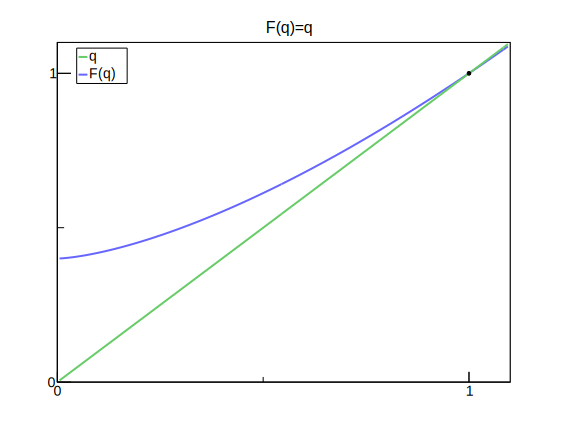
\includegraphics[width=0.4\textwidth]{./Immagini/Teoria/banale}}
	$\;$
	\subfloat[Esistenza di $q<1$]
	{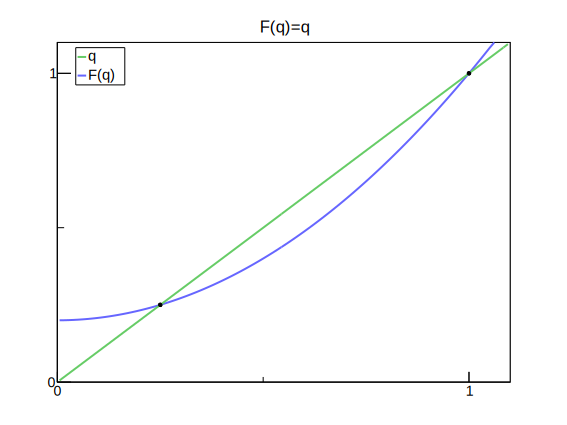
\includegraphics[width=0.4\textwidth]{./Immagini/Teoria/nonbanale}}
	\caption[Esistenza soluzione non banale.]{Confronto tra il caso in cui $F(q)=q$ ha solo la soluzione banale $q=1$, e il caso in cui esiste una soluzione per $q<1$.}
	\label{fig:banalita}
\end{figure}

\begin{equation}
\label{eq:condizione}
	q = \sum_k P_{\rightarrow}(k) q^{k-1},
\end{equation}
Se definiamo a sua volta $P_{\rightarrow}(k)$ come la probabilit\`a di avere un nodo di grado $k$, per il numero di link possibili con cui possiamo ottenerlo (cio\`e il suo grado), allora $P_{\rightarrow}(k)$ diventa
\[P_{\rightarrow}(k) = \frac{P(k)k}{\sum_{k'}P(k')k'} = \frac{P(k)k}{\langle k \rangle}\]
\[\Rightarrow q = \frac{1}{\langle k \rangle}\sum_k P(k)kq^{k-1} \]
Questa \`e uan funzione parametrica e ricorsiva. Chiamandola $F(q)$ e studiandola si ha che ha derivate prima e seconda positive, pertanto \`e sempre crescente e convessa; inoltre si ha che $F(1) = 1$ e $F(0)>0$. Tutto ci\`o vale per qualsiasi parametro $k$. 

Risolvendo l'equazione $q = F(q)$ si ottiene la condizione secondo cui il giant cluster non pu\`o esistere. Infatti, se esiste una soluzione oltre a quella banale per $q=1$, significa che l'equazione \ref{eq:condizione} \`e verificata per valori di $q<1$ e che quindi il giant cluster esiste. Come si pu\`o vedere dalla figura \ref{fig:banalita}, si pu\`o adottare un metodo grafico: la retta e la curva si intersecano sempre in due punti, il primo con $F'(q)<q'=1$ e il secondo con $F'(q) \geq 1$. Dato che uno dei due deve sempre essere $F(1)=1$, se 

$$F'(q=1) \geq 1 $$
significa che esiste un altro punto di intersezione per $q<1$ e quindi esiste il giant cluster.
Svolgendo $d_qF|_{q=1} \geq 1$ si ottiene la condizione di esistenza dello spanning cluster in termini del grado, o criterio di \textcite{Molloy1995}:

\begin{equation}
\label{eq:criterion}
	\frac{\langle k^2\rangle}{\langle k \rangle}\geq 2.
\end{equation}



Questo risultato \`e valido per ogni tipo di rete \parencite{Cohen2000}. Un nodo con un grado iniziale $k_0$ avr\`a, dopo la rimozione di una frazione $f$ di nodi, un grado k con una probabilit\`a dettata da una distribuzione binomiale $B_{p,k_0}(k)$, e quindi la nuova distribuzione dei gradi sar\`a $P(k) = \sum_{k_0} P(k_0)B_{p,k_0}(k)$. Ricavando i nuovi $\langle k \rangle$ e $\langle k^2 \rangle$ si ottiene che la frazione di nodi rimossi necessaria perch\'e si verifichi che $\langle k^2\rangle/\langle k \rangle = 2$, e cio\`e il grafo sia completamente frammentato, \`e 
\begin{equation}
\label{eq:criterionfreq}
	f = 1 - \frac{1}{\frac{\langle k^2 \rangle}{\langle k \rangle}-1}
\end{equation}

Nel caso specifico di una rete costruita con il modello di Barabasi-Albert, questa avr\`a $P(k)\propto k^{-\alpha}$, che spazier\`a da un minimo $m$ e un massimo $K$. In questo caso, ponendo $K\gg m \gg 1$, si pu\`o approssimare $k$ a una grandezza continua e si ottengono due comportamenti a seconda del valore di $\alpha$:
 \[\frac{\langle k^2\rangle}{\langle k \rangle} = c \frac{2-\alpha}{3-\alpha},\]
 con
\begin{description}
	\item[$\alpha > 3 \Rightarrow c\sim m.$] Si ha una transizione allo stato completamente frammentato per valori di $f<1$
	\item[$\alpha < 3 \Rightarrow c=c(K).$] La transizione dipende dal valore di $K$, per cui esiste per reti finite, ma per $K \rightarrow \infty$ $f\rightarrow1$.
\end{description}

Nel caso dell'attacco intenzionale la percentuale $f$ \`e ottenuta per via numerica. Dato inoltre il peculiare metodo di attacco scelto, sarebbe necessario uno studio progressivo che a ogni iterazione tenga conto del taglio dei $k$ pi\`u grandi e ricalcoli la $P(k)$ per ottenere il rapporto $\frac{\langle k^2 \rangle}{\langle k \rangle}$. Risulterebbe pertanto pi\`u conveniente effettuare simulazioni numeriche direttamente sui modelli \parencite{Cohen2001}.

In ogni caso, a livello qualitativo, come nel caso di attacco random ci si aspettava una maggiore resistenza da parte delle reti scale-free, a causa del grande numero di nodi poco connessi che garantisce una $P(k)$ a legge di potenza con un opportuno $\alpha$, nel caso dell'attacco intenzionale ci si aspetta una certa fragilit\`a. Infatti le reti scale free sono costruite attorno ai nodi pi\`u connessi, si pu\`o supporre quindi che rimuoverli per primi provochi un deterioramento pi\`u veloce rispetto a una rete random con uguale grado medio \parencite{Barbalbert2002}.

